% Chapter 5
\chapter{THỰC NGHIỆM, ĐÁNH GIÁ VÀ THẢO LUẬN} % Main chapter title
\label{Chapter4}

\section*{Tóm tắt chương}
Trong chương này, chúng tôi sẽ trình bày chi tiết cách hiện thực hóa phương pháp đã trình bày trong \textbf{Chương \ref{Chapter3}}, đồng thời, chúng tôi trình bày cách xây dựng môi trường thực nghiệm, kịch bản và các kết quả đạt được khi thực nghiệm công cụ.
\newline

\section{Môi trường thực nghiệm}

\begin{itemize}
    \item \textbf{Máy local}
    \begin{itemize}
        \item CPU: Intel\textregistered{} Core\texttrademark{} i7-8565u (4 cores - 1.8 GHz)
        \item RAM: 16GB
        \item OS: Windows 11
        \item Dung lượng ổ đĩa: 512GB
    \end{itemize}
    Máy local được sử dụng để triển khai hệ thống tự động quá quá trình săn tìm mối đe dọa.
    
    \item \textbf{Máy ảo Vcenter}
    \begin{itemize}
        \item CPU: Intel\textregistered{} Xeon\texttrademark{} E5-2660 (6 cores - 1.0 Ghz)
        \item RAM: 64GB
        \item OS: Ubuntu 20.04
        \item Dung lượng ổ đĩa: 100GB
    \end{itemize}
    Máy ảo Vcenter được chúng tôi sử dụng để thực nghiệm các kịch bản huấn luyện các hệ thống phát hiện tấn công APT sử dụng học liên kết.

    \item \textbf{Môi trường phát triển}
    \begin{itemize}
        \item Trình soạn thảo: Visual Studio Code.
        \item Ngôn ngữ lập trình: Python3, Go.
        \item Thư viện sử dụng: numpy, pandas, mathplotlib, sklearn, tensorflow, torch.
        \item Nền tảng Federated Learing: Tensorflow, PyTorch.
    \end{itemize}
\end{itemize}


\section{Xây dựng mô hình học liên kết cho các hệ thống phát hiện tấn công APT} \label{sec:implemented-FL-based-IDS}

\subsection{Tập dữ liệu}

Để kiểm tra tính hiệu quả của hai mô hình IDS đề xuất được huấn luyện dựa trên phương pháp học liên kết, chúng tôi sử dụng hai bộ dữ liệu lần lượt là bộ dữ liệu NF-ToN-IoT và DARPA Transparent Computing Engagement 3 (TCE3)\footnote{DARPA TCE3: \url{https://github.com/darpa-i2o/Transparent-Computing/blob/master/README-E3.md}}. Bộ dữ liệu NF-ToN-IoT được sử dụng để huấn luyện và kiểm tra hiệu năng của NIDS trong việc cho việc phát hiện \textit{flow} bất thường trong mạng SDN và bộ dữ liệu TCE3 được sử dụng để huấn luyện và kiểm tra hiệu năng của PIDS trong việc phát hiện các hành vi bất thường trong đồ thị nguồn gốc được tạo bởi các \textit{log} trên các điểm đầu cuối.

\bigbreak\noindent
Bộ dữ liệu NF-ToN-IoT được xây dựng dựa trên giao thức NetFlow \cite{sarhan2020netflow} là một phần của tập các bộ dữ liệu NetFlow v1\footnote{Các bộ dữ liệu cho NIDS: \url{https://staff.itee.uq.edu.au/marius/NIDS_datasets}} (bao gồm 5 bộ dữ liệu: NF-ToN-IoT, NF-UNSW-NB15, NF-UQ-NIDS, NF-BoT-IoT và NF-CSE-CIC-IDS2018. Các bộ dữ liệu trong tập NetFlow v1 có 12 thuộc tính NetFlow được liệt kê trong \textbf{Bảng \ref{tab:flow-features}} và chứa các loại tấn công khác nhau như DDoS, backdoor, quét mạng, ... Bộ dữ liệu NF-ToN-IoT được sử dụng để huấn luyện và kiểm tra hiệu năng của mô hình NIDS có tổng cộng 1,379,274 bản ghi, trong đó có 1,108,995 (80,4\%) bản ghi là độc hại và 270,279 (19,6\%) bản ghi là lành tính.

\bigbreak\noindent
Bộ dữ liệu DARPA TCE3 được đặt theo tên của một thực nghiệm mô phỏng các cuộc tấn công APT được thực hiện trên một hệ thống bao gồm nhiều máy chủ với các hệ điều hành khác nhau. Các hoạt động và sự kiện trong hệ thống được giám sát và ghi lại dưới dạng \textit{log}. Trong thực nghiệm này, chúng tôi sử dụng dữ liệu \textit{log} được thu thập từ máy chủ CADETS FreeBSD để đánh giá hiệu suất của mô hình PIDS đề xuất. Bộ dữ liệu được thu thập từ máy chủ CADETS FreeBSD bao gồm 13.880.763 sự kiện, bao gồm các hoạt động lành tính hàng ngày của hệ thống và các hoạt động tấn công do Drakon APT gây ra bằng cách sử dụng lỗ hổng Nginx backdoor. Tuy nhiên, do số lượng sự kiện lành tính là quá lớn nên thay vì sử dụng tất cả các sự kiện có trong tập dữ liệu, chúng tôi quyết định loại bỏ các sự kiện được biết chắc là lành tính và không có liên hệ nào với các sự kiện còn lại để tạo ra một bộ dữ liệu với tổng cộng 237,721 sự kiện, trong đó có 236,160 (99.3\%) sự kiện là lành tính và 1,561 (0.7\%) sự kiện là độc hại.
\bigbreak\noindent
Phân phối dữ liệu của hai tập dữ liệu được tóm tắt trong bảng sau:

\begin{table}[h]
\centering
\caption{Phân bố dữ liệu của hai tập dữ liệu}
\begin{tabular}{|c|c|c|c|}
\hline
           & Lành tính        & Độc hại            & Tổng số   \\ \hline
NF-ToN-IoT & 270,279 (19,6\%) & 1,108,995 (80,4\%) & 1,379,274 \\ \hline
DARPA TCE3 & 236,160 (99.3\%) & 1,561 (0.7\%)      & 237,721   \\ \hline
\end{tabular}
\end{table}


\subsection{Tiền xử lý dữ liệu}

\textbf{Bộ dữ liệu NF-ToN-IoT:} Để đảm bảo mô hình đề xuất không phụ thuộc vào các thuộc tính không mong muốn, chúng tôi đã loại bỏ địa chỉ IP nguồn-đích. Sau đó, chúng tôi cũng áp dụng công thức chuẩn hóa đặc trưng cho từng thuộc tính và công thức nào được sử dụng cho thuộc tính nào được chúng tôi đề cập trong \textbf{bảng \ref{tab:flow-features}}. Trong đó, công thức chuẩn hóa đặc trưng đầu tiên được sử dụng là chuẩn hóa $min-max$, được áp dụng để chuyển đổi giá trị các thuộc tính về khoảng [0,1] như sau:

\begin{equation} \label{eq:mix&max-normalized}
    x_{normalized} = \frac{x-x_{min}}{x_{max}-x_{min}}
\end{equation}

\bigbreak\noindent
trong đó $x_{min}=0$, $x_{max}=256^{feature\_size}-1$ với $feature\_size$ là kích thước của thuộc tính tương ứng được hiển thị trong \textbf{Bảng \ref{tab:flow-features}}, và $x$ là giá trị của thuộc tính hiện tại.

\bigbreak\noindent
Trong công thức thứ hai, chúng tôi sử dụng phương pháp chuẩn hóa được đề xuất bởi Raskovalov và các cộng sự \cite{raskovalov2022investigation} để tối ưu hóa sự linh hoạt của quá trình chuẩn hóa trên các thuộc tính có giá trị nằm trong phạm vi lớn. Công thức được định nghĩa như sau:

\begin{equation} \label{eq:erf-normalized}
    x_{normalized} = erf(\frac{x}{k_w})
\end{equation}

\bigbreak\noindent
trong đó $k_w$ là hệ số chuẩn hóa tương ứng được hiển thị trong \textbf{Bảng \ref{tab:flow-features}}, $erf(x)= \frac{2}{\sqrt{\pi}} \int_{0}^{x} e^{-t^2} \, dt$ (hàm lỗi Gauss), và $x$ là giá trị của thuộc tính hiện tại.

\begin{table}[ht]
    \centering
    \caption{Phương pháp chuẩn hoá cho từng loại thuộc tính của \textit{flow}.}
    \label{tab:flow-features}
    \begin{adjustbox}{width=\textwidth}
    \begin{threeparttable}
    \begin{tabular}{|c|c|c|c|c|c|}
    \hline
    \textbf{Thuộc tính} & \textbf{Kích thước} & \makecell{\textbf{Phương pháp}\\\textbf{chuẩn hoá}} & \makecell{\textbf{Hệ số chuẩn hoá $k_w$}} \\
    \hline
    \texttt{IPV4\_SRC\_ADDR} & 4 bytes & - & -\\
    \hline
    \texttt{IPV4\_DST\_ADDR} & 4 bytes & - & - \\
    \hline
    \texttt{PROTOCOL} & 1 bytes & \eqref{eq:mix&max-normalized} & - \\
    \hline
    \texttt{L4\_SRC\_PORT} & 2 bytes & \eqref{eq:mix&max-normalized} & - \\
    \hline
    \texttt{L4\_DST\_PORT} & 2 bytes & \eqref{eq:mix&max-normalized} & - \\
    \hline
    \texttt{IN\_PKTS} & 4 bytes & \eqref{eq:erf-normalized} & 20 \\
    \hline
    \texttt{OUT\_PKTS} & 4 bytes & \eqref{eq:erf-normalized} & 20 \\
    \hline
    \texttt{IN\_BYTES} & 4 bytes & \eqref{eq:erf-normalized} & 900 \\
    \hline
    \texttt{OUT\_BYTES} & 4 bytes & \eqref{eq:erf-normalized} & 900 \\
    \hline
    \texttt{TCP\_FLAGS} & 1 bytes & \eqref{eq:mix&max-normalized} & - \\
    \hline
    \texttt{FLOW\_DURATION\_MILLISECONDS} & 4 bytes & \eqref{eq:erf-normalized} & 600 \\
    \hline
    \texttt{L7\_PROTO} & 2 bytes & \eqref{eq:mix&max-normalized} & - \\
    \hline
    \end{tabular}
    \end{threeparttable}
    \end{adjustbox}
\end{table}

\bigbreak\noindent
\textbf{Bộ dữ liệu DARPA TCE3}: Bao gồm các đối tượng và sự kiện. Trong đó, các đối tượng gồm các thực thể tồn tại trên máy chủ, chẳng hạn như tệp tin, thư mục và các ống không đặt tên (thường được sử dụng để giao tiếp và chia sẻ tài nguyên giữa các tiến trình). Các đối tượng này sẽ được biểu diễn là một nút trong đồ thị nguồn gốc và một sự kiện là một cạnh biểu diễn mối liên hệ giữa hai nút. Các sự kiện giữa hai nút có thể là chỉnh sửa, xóa, tạo, thực thi, ... Sau khi tạo ra đồ thị ban đầu, các thuộc tính của các đối tượng sẽ được chuyển đổi thành câu có thể xử lý được bởi mô hình Transformer. Cấu trúc câu chuyển đổi cho các loại đối tượng được thể hiện thông qua \textbf{Bảng \ref{tab:dataset-node-preprocessing}}.


\begin{table}[ht]
    \centering
    \caption[Mẫu câu cho từng loại đối tượng.]{Mẫu câu cho từng loại đối tượng. Các thuộc tính của đối tượng được biểu diễn trong hai ngoặc nhọn, và sẽ được thay thế cùng với các dấu ngoặc nhọn thành giá trị khi chuyển thành câu.}
    \label{tab:dataset-node-preprocessing}
    \begin{adjustbox}{width=0.9\textwidth}
    \begin{threeparttable}
    \begin{tabular}{|c|c|}
    \hline
    \textbf{Loại đối tượng} & \textbf{Mẫu câu} \\
    \hline
    \texttt{net\_flow} & \makecell{A net flow object\\had the local address of \{\{{\texttt{local\_address}}\}\}:\{\{\texttt{local\_port}\}\}\\and the remote address of \{\{\texttt{remote\_address}\}\}:\{\{\texttt{remote\_port}\}\}} \\
    \hline
    \texttt{file} & \makecell{A file object had the subtype named \{\{\texttt{sub\_type}\}\}} \\
    \hline
    \texttt{subject} & \makecell{A subject object had the subtype named \{\{\texttt{sub\_type}\}\}} \\
    \hline
    \texttt{unnamed\_pipe} & \makecell{An unnamed piped object had no properties} \\
    \hline
    \end{tabular}
    \end{threeparttable}
    \end{adjustbox}
\end{table}

\bigbreak\noindent
%Tuy nhiên, trong quá trình Khi xử lý bộ dữ liệu DARPA TCE3, chúng tôi gặp hai vấn đề chính. Thứ nhất, do số lượng sự kiện độc hại rất nhỏ, việc sử dụng toàn bộ tập dữ liệu có thể gây ra vấn đề hiệu suất huấn luyện mô hình. Nên thay vì chọn tất cả các sự kiện có trong tập dữ liệu, chúng tôi quyết định chọn một tập con cụ thể chứa phần lớn các sự kiện độc hại, với tổng cộng 237,721 sự kiện, trong đó có 236,160 (99.3\%) sự kiện là lành tính và 1,561 (0.7\%) sự kiện là độc hại.

\bigbreak\noindent
%Thứ hai, mô hình GraphSAGE gặp khó khăn trong việc phân tích các mối liên hệ giữa các đối tượng do chỉ tập trung vào thông tin được cung cấp bởi các đối tượng. %Trong khi, hầu hết các đối tượng trong tập dữ liệu có đặc trưng quá đơn giản như là \texttt{type} và \texttt{sub\_type}.
Ngoài ra, để tránh trường hợp mô hình GraphSAGE thiếu thông tin về mối liên hệ giữa các đối tượng do chỉ có thể sử dụng thông tin được cung cấp bởi các nút, chúng tôi sử dụng các câu của đối tượng kết hợp với thuộc tính của các sự kiện tương ứng để tạo thành câu hoàn chỉnh cho mỗi nút trong đồ thị. Các câu được tạo thành sẽ có cấu trúc khác nhau tùy thuộc vào vai trò của đối tượng là nguồn hay đích của sự kiện. Ví dụ, một câu cho một nút nguồn ở dạng \textit{file} đang thực thi (\textit{execute}) một lệnh lên một đối tượng khác: ``\textit{A file object had the subtype named file, and it executed bash with the command line ``rm a.txt"}". Sau khi tạo câu cho tất cả các nút trong đồ thị, chúng tôi sử dụng mô hình \emph{sentence\_transformers} \cite{reimers-2019-sentence-bert} đã được huấn luyện trước có tên là \emph{all-MiniLM-L6-v2} \cite{reimers-2020-multilingual-sentence-bert} để biến đổi các câu thành các vectơ có kích thước cố định.
%\bigbreak\noindent
%Để chứng minh tính hiệu quả của việc tích hợp đặc trưng nút, chúng tôi so sánh chúng với đặc trưng nút độc lập trong \textcolor{red}{??????????}.

\begin{table}[ht]
    \centering
    \caption[Mẫu chuỗi từ cho sử dụng để kết hợp với câu của đối tượng]{Mẫu chuỗi từ cho sử dụng để kết hợp với câu của đối tượng. Các thuộc tính của sự kiện được biểu diễn trong hai ngoặc nhọn, và sẽ được thay thế cùng với các dấu ngoặc nhọn thành giá trị khi chuyển thành chuỗi từ}
    \label{tab:dataset-edge-preprocessing}
    \begin{adjustbox}{width=\textwidth}
    \begin{threeparttable}
    \begin{tabular}{|c|c|c|c|}
    \hline
    \textbf{Loại sự kiện} & \makecell{\textbf{Mẫu phần đầu chuỗi từ nếu}\\\textbf{kết hợp với nút nguồn}\\} & \makecell{\textbf{Mẫu phần đầu chuỗi từ nếu}\\\textbf{kết hợp với nút đích}\\} & \textbf{Mẫu phần sau chuỗi từ} \\
    \hline
    \texttt{execute} & executed & was executed using & \makecell{\{\{\texttt{exec}\}\} with the\\command line ``\{\{\texttt{cmd\_line}\}\}"} \\
    \hline
    \texttt{accept} & \makecell{accepted the\\connection from} & \makecell{was accepted to connect\\with the address} & \makecell{\{\{\texttt{address}\}\} using \{\{\texttt{exec}\}\}} \\
    \hline
    \texttt{create\_object} & created an object & was created & \makecell{using \{\{\texttt{exec}\}\}} \\
    \hline
     \texttt{modify\_process} & modified a process & was modified & \makecell{using \{\{\texttt{exec}\}\}} \\
     \hline
     \texttt{rename} & renamed an object & was renamed & \makecell{using \{\{\texttt{exec}\}\}} \\
     \hline
     \texttt{add\_attributes} & \makecell{added attributes to an object} & \makecell{attributes was added} & - \\
     \hline
     \texttt{flows\_to} & flowed & was flowed & to another object \\
    \hline
    \end{tabular}
    \end{threeparttable}
    \end{adjustbox}
\end{table}



\subsection{Cấu hình}

Chúng tôi mô phỏng quá trình huấn luyện các mô hình IDS sử dụng học liên kết với 10 máy khách trong 10 vòng. Cấu trúc chi tiết của mô hình GRU\&CNN và mô hình TGraphSAGE được mô tả lần lượt trong \textbf{Bảng \ref{tab:cnn-gru-model-architecture}} và \textbf{Bảng \ref{tab:graphsage-model-architecture}}. 

\begin{table}[h]
    \centering
    \caption{Kiến trúc của mô hình GRU\&CNN}
    \label{tab:cnn-gru-model-architecture}
    \scalebox{1}{
    \begin{threeparttable}
    \begin{tabular}{|c|c|c|c|}
    \hline
    \textbf{Lớp (ID)} & \textbf{Hàm kích hoạt} & \textbf{Kích thước đầu ra} &\textbf{ Kết nối với}  \\
    \hline
    Input (1) & - & $(10, 1)$ & [] \\
    \hline
    Conv1D (2) & ReLU & $(10, 32)$ & [(1)] \\
    \hline
    BatchNormalization (3) & - & $(10, 32)$ & [(2)] \\
    \hline
    MaxPooling1D (4) & - & $(10, 32)$ & [(3)] \\
    \hline
    Conv1D (5) & ReLU & $(10, 32)$ & [(4)] \\
    \hline
    BatchNormalization (6) & - & $(10, 32)$ & [(5)] \\
    \hline
    MaxPooling1D (7) & - & $(10, 32)$ & [(6)] \\
    \hline
    Conv1D (8) & ReLU & $(10, 32)$ & [(7)] \\
    \hline
    Batch Normalization (9) & - & $(10, 32)$ & [(8)] \\
    \hline
    MaxPooling1D (10) & - & $(10, 32)$ & [(9)] \\
    \hline
    Global Max Pooling (11) & - & $(32)$ & [(10)] \\
    \hline
    GRU (12) & - & $(32)$ & [(1)] \\
    \hline
    Concatenate (13) & - & $(64)$ & [(11), (12)] \\
    \hline
    Dense (14) & - & $(32)$ & [(13)] \\
    \hline
    Dense (15) & Sigmoid & $(1)$ & [(14)] \\
    \hline
    \end{tabular}
    \end{threeparttable}}
\end{table}

\begin{table}[ht]
    \centering
    \caption{Kiến trúc của mô hình TGraphSAGE}
    \label{tab:graphsage-model-architecture}
    \scalebox{1}{
    \begin{tabular}{|c|c|c|c|}
    \hline
    \textbf{Lớp (ID)} & \textbf{Hàm kích hoạt} & \textbf{Kích thước đầu ra} &\textbf{ Kết nối với}  \\
    \hline
%    Input (1) & \makecell{Node: (1, 384)\\Edge: (1, 384)} & [] \\
    Input (1) & - & $(384)$ & - \\
    \hline
    SAGELayer (2) & ReLU & $(256)$ & (1) \\
    \hline
    SAGELayer (3) & ReLU & $(256)$ & (2) \\
    \hline
    SAGELayer (4) & ReLU & $(128)$ & (3) \\
    \hline
    SAGELayer (5) & - & $(2)$ & (4) \\
    \hline
    \end{tabular}}
\end{table}

\bigbreak\noindent
Ngoài ra, dựa trên các kết quả thực nghiệm trước đây của chúng tôi và các công trình có liên quan, chúng tôi thực hiện huấn các mô hình cục bộ trên các máy khách với cấu hình sau: sử dụng thuật toán tối ưu $Adam$ với $learning\_rate=0.001$, $epoch=5$ và $batch\_size=512$ cho mô hình GRU\&CNN, và cấu hình tương tự được áp dụng cho mô hình TGraphSAGE nhưng với $epoch=100$ và không sử dụng dụng $batch\_size$. Bên cạnh đó, chúng tôi sử dụng 70\% dữ liệu để huấn luyện các máy khách và 30\% còn lại cho việc đánh giá, đồng thời đảm bảo tỷ lệ mẫu độc hại và lành tính trong quá trình chia để ngăn việc mất cân bằng trong quá trình đánh giá. Cách chia trên được chúng tôi áp dụng cho cả hai tập dữ liệu NF-ToN-IoT và tập dữ liệu DARPA TCE3. Cuối cùng, các tập dữ liệu huấn luyện sẽ được chia đều và phân phối cho tất cả các máy khách.

\subsection{Tiêu chí đánh giá dự đoán của các mô hình IDS} \label{sec:detection-metric}
Để đánh giá dự đoán của mô hình một cách phù hợp, chúng tôi đã thảo luận và định nghĩa các giá trị đầu ra có thể có của mô hình như sau: \textit{true positive} (TP) đại diện cho số lượng dự đoán chính xác thuộc lớp tấn công, \textit{true negative} (TN) đại diện cho số lượng dự đoán chính xác thuộc lớp lành tính, \textit{false positive} (FP) đại diện cho số lượng nhãn bình thường bị phân loại sai vào lớp tấn công, \textit{false negative} (FN) đại diện cho số lượng nhãn tấn công bị phân loại sai vào lớp lành tính.
\bigbreak\noindent
Dựa trên các giá trị trên, chúng tôi sử dụng bốn tiêu chí sau để đánh giá hiệu suất của các mô hình IDS:

\begin{itemize}
    \item \emph{Accuracy} là tỷ lệ giữa số lượng dự đoán đúng và tổng số dự đoán.
    \begin{equation} \label{eq:accuracy}
        Accuracy = \frac{TP + TN}{TP + TN + FP + FN}
    \end{equation}
    \item \emph{Precision} là tỷ lệ giữa số lượng dự đoán đúng thuộc lớp tấn công và tổng số dự đoán thuộc lớp tấn công.
    \begin{equation} \label{eq:precision}
        Precision = \frac{TP}{TP + FP}
    \end{equation}
    \item \emph{Recall} là tỷ lệ giữa số lượng dự đoán đúng có nhãn tấn công và tổng số lượng dự đoán đúng có nhãn tấn công cộng với số lượng dự đoán bị phân loại sai thuộc lớp bình thường.
    \begin{equation} \label{eq:recall}
        Recall = \frac{TP}{TP + FN}
    \end{equation}
    \item \emph{F1-score} được tính bằng hai lần tích của \emph{precision} và \emph{recall} chia cho tổng của \emph{precision} và \emph{recall}.
    \begin{equation} \label{eq:f1-score}
        F1-score = 2 \cdot \frac{Recall \cdot Precision}{Recall + Precision}
    \end{equation}
\end{itemize}

\subsection{Kết quả thực nghiệm và nhận xét} 

\textbf{Bảng \ref{tab:detection-metric-result}} hiển thị kết quả huấn luyện của mô hình GRU\&CNN trên bộ dữ liệu NF-ToN-IoT và mô hình TGraphSAGE trên bộ dữ liệu DARPA TCE3, được đánh giá theo các tiêu chí đã được đề cập trong \textbf{Mục \ref{sec:detection-metric}}. Nhìn chung, chúng ta có thể thấy rằng cả hai mô hình được đề xuất cho NIDS và PIDS đều đạt được hiệu suất rất cao, tất cả đều trên 0.9. Trong đó, chỉ số có giá trị thấp nhất của mô hình GRU\&CNN là 0.9962 và giá trị thấp nhất cho mô hình TGraphSAGE là 0.9173 (khi chỉ sử dụng thuộc tính của nút). Hơn thế nữa, Mô hình TGraphSAGE có hiệu suất tổng thể cao hơn mô hình GraphSAGE sử dụng doc2vec \cite{le2014distributed}, word2vec \cite{church2017word2vec} và fasttext \cite{bojanowski2017enriching} trong việc xử lý dữ liệu từ đồ thị. Ngoài ra, mặc dù bộ dữ liệu DARPA TCE3 mất cân bằng một cách nghiêm trọng với các mẫu lành tính chiếm tới 99.3\%, mô hình TGraphSAGE và mô hình GraphSAGE tích hợp fasttext vẫn đạt được giá trị tuyệt đối trong tiêu chí \textit{Recall} (1.0). Điều này cho thấy hiệu suất ấn tượng của TGraphSAGE và mô hình GraphSAGE tích hợp fasttext trong việc phát hiện các sự kiện độc hại, đặc biệt là trong trường hợp các sự kiện này chiếm số lượng rất nhỏ so với các sự kiện lành tính xảy ra hàng ngày trong hệ thống. Tuy nhiên, mô hình đề xuất của chúng tôi nhỉnh hơn về chỉ số \textit{Precision} nên cho ra tỷ lệ dương tính giả thấp hơn. Cuối cùng, chúng tôi còn so sánh mô hình GRU\&CNN được đề xuất với mô hình DeepFed và mô hình được thay thế mô-đun GRU bằng LSTM. Cả ba mô hình đều cho kết quả huấn luyện tương đương nhau nhưng mô hình DeepFed cho thời gian huấn luyện lâu nhất và mô hình GRU\&CNN cho kết quả nhanh nhất.


\begin{table}[h]
    \centering
    \caption[Kết quả đánh giá hiệu suất của các mô hình được đề xuất]{Kết quả đánh giá hiệu suất của mô hình GRU\&CNN và mô hình TGraphSAGE}
    \label{tab:detection-metric-result}
\begin{tabular}{|c|c|c|c|c|c|}
\hline
                      & \textbf{Model}                                                                & \textbf{Accuracy} & \textbf{Precision} & \textbf{Recall} & \textbf{F1-Score} \\ \hline
\multirow{3}{*}{NIDS} & DeepFed                                                                       & 0.9982            & 0.9985             & 0.9993          & 0.9989            \\ \cline{2-6} 
                      & LSTM\&CNN                                                                     & 0.998             & 0.9983             & 0.9993          & 0.9988            \\ \cline{2-6} 
                      & \textbf{GRU\&CNN}                                                             & \textbf{0.9982}   & \textbf{0.9985}    & \textbf{0.9992} & \textbf{0.9989}   \\ \hline
\multirow{5}{*}{PIDS} & doc2vec+GraphSAGE                                                                 & 0.9976            & 0.9587             & 0.5946          & 0.7339            \\ \cline{2-6} 
                      & word2vec+GraphSAGE                                                                 & 0.9992            & 0.8824             & 0.9984          & 0.9368            \\ \cline{2-6} 
                      & fasttext+GraphSAGE                                                            & 0.9995            & 0.9258             & 1.0               & 0.9615            \\ \cline{2-6} 
                      & \begin{tabular}[c]{@{}c@{}}TGraphSAGE\\      (node feature only)\end{tabular} & 0.9995            & 0.9173             & 0.9952          & 0.9547            \\ \cline{2-6} 
                      & \textbf{TGraphSAGE}                                                           & \textbf{0.9996}   & \textbf{0.9313}    & \textbf{1.0}      & \textbf{0.9645}   \\ \hline
\end{tabular}
\end{table}

\bigbreak\noindent
Bên cạnh đó, phương pháp sử dụng cả thuộc tính của nút và cạnh được đề xuất giúp quá trình huấn luyện sử dụng học liên kết hội tụ nhanh hơn và đạt hiệu suất tốt nhất từ vòng 3 (như được mô tả trong \textbf{Hình \ref{fig:node&edge}}). Trong khi đó, phương pháp truyền thống (chỉ sử dụng thuộc tính của nút) cho hiệu suất không ổn định cho đến vòng huấn luyện cuối cùng (như được mô tả trong \textbf{Hình \ref{fig:node}}).


\begin{figure}[h]%
 \centering
 \subfloat[]{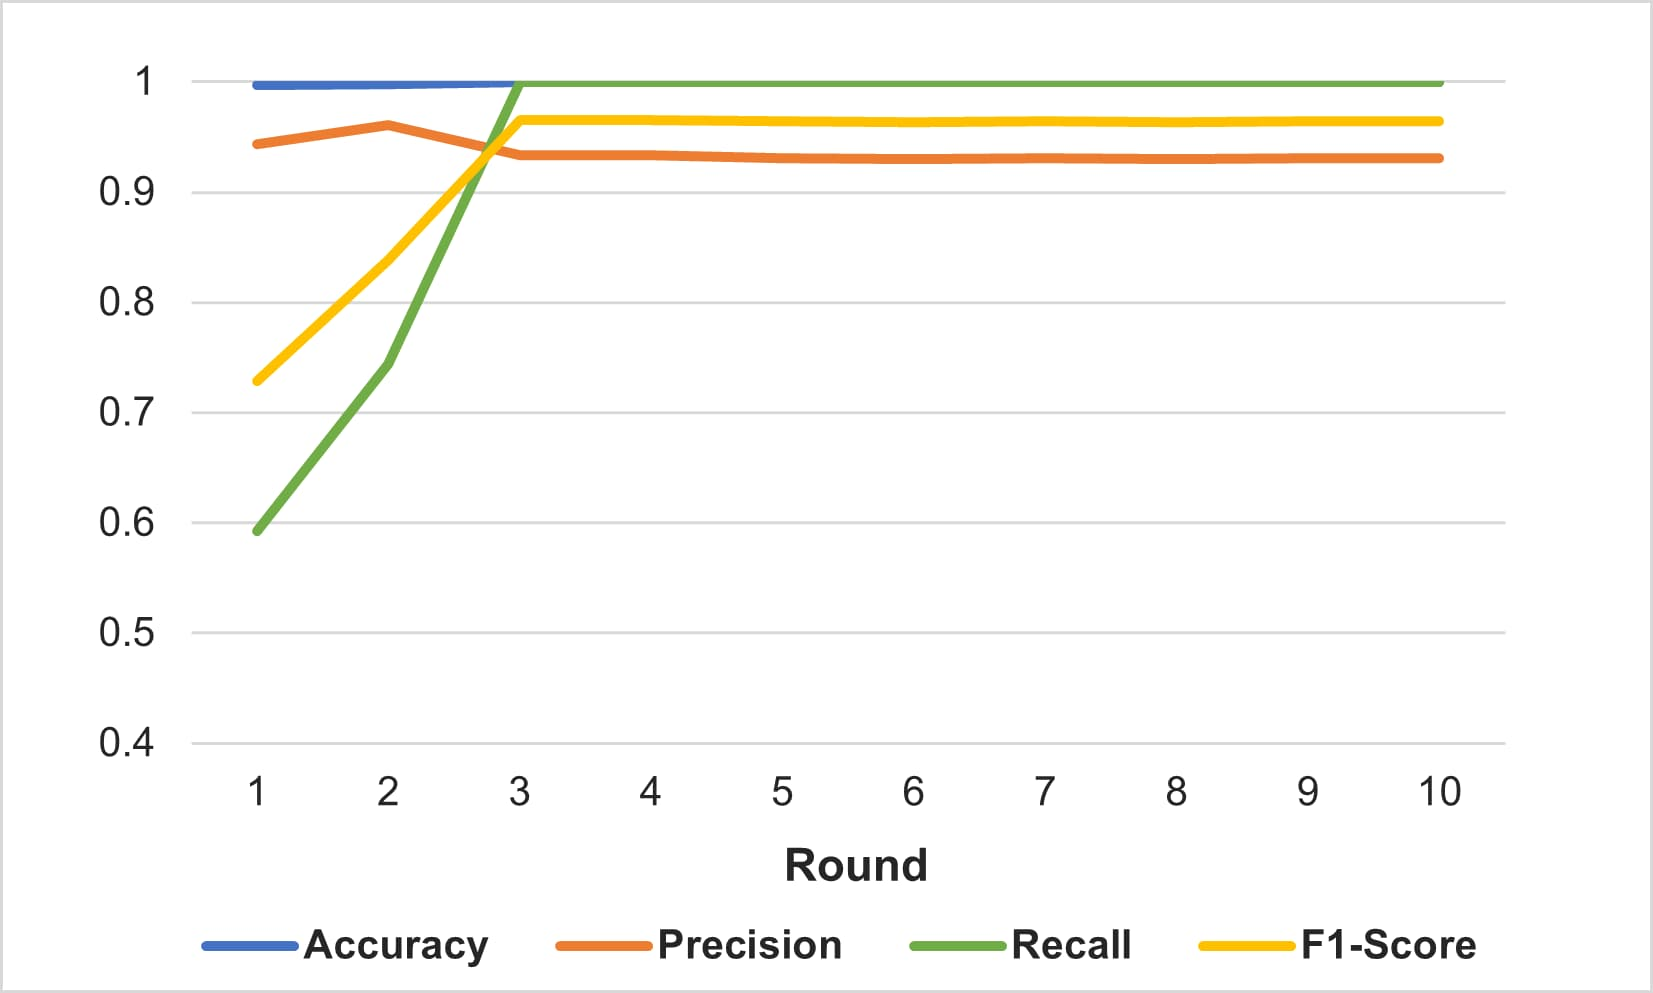
\includegraphics[width=0.5\linewidth]{src/images/chapter4/Node-Edge-GraphSAGE.jpg}\label{fig:node&edge}}%
 \subfloat[]{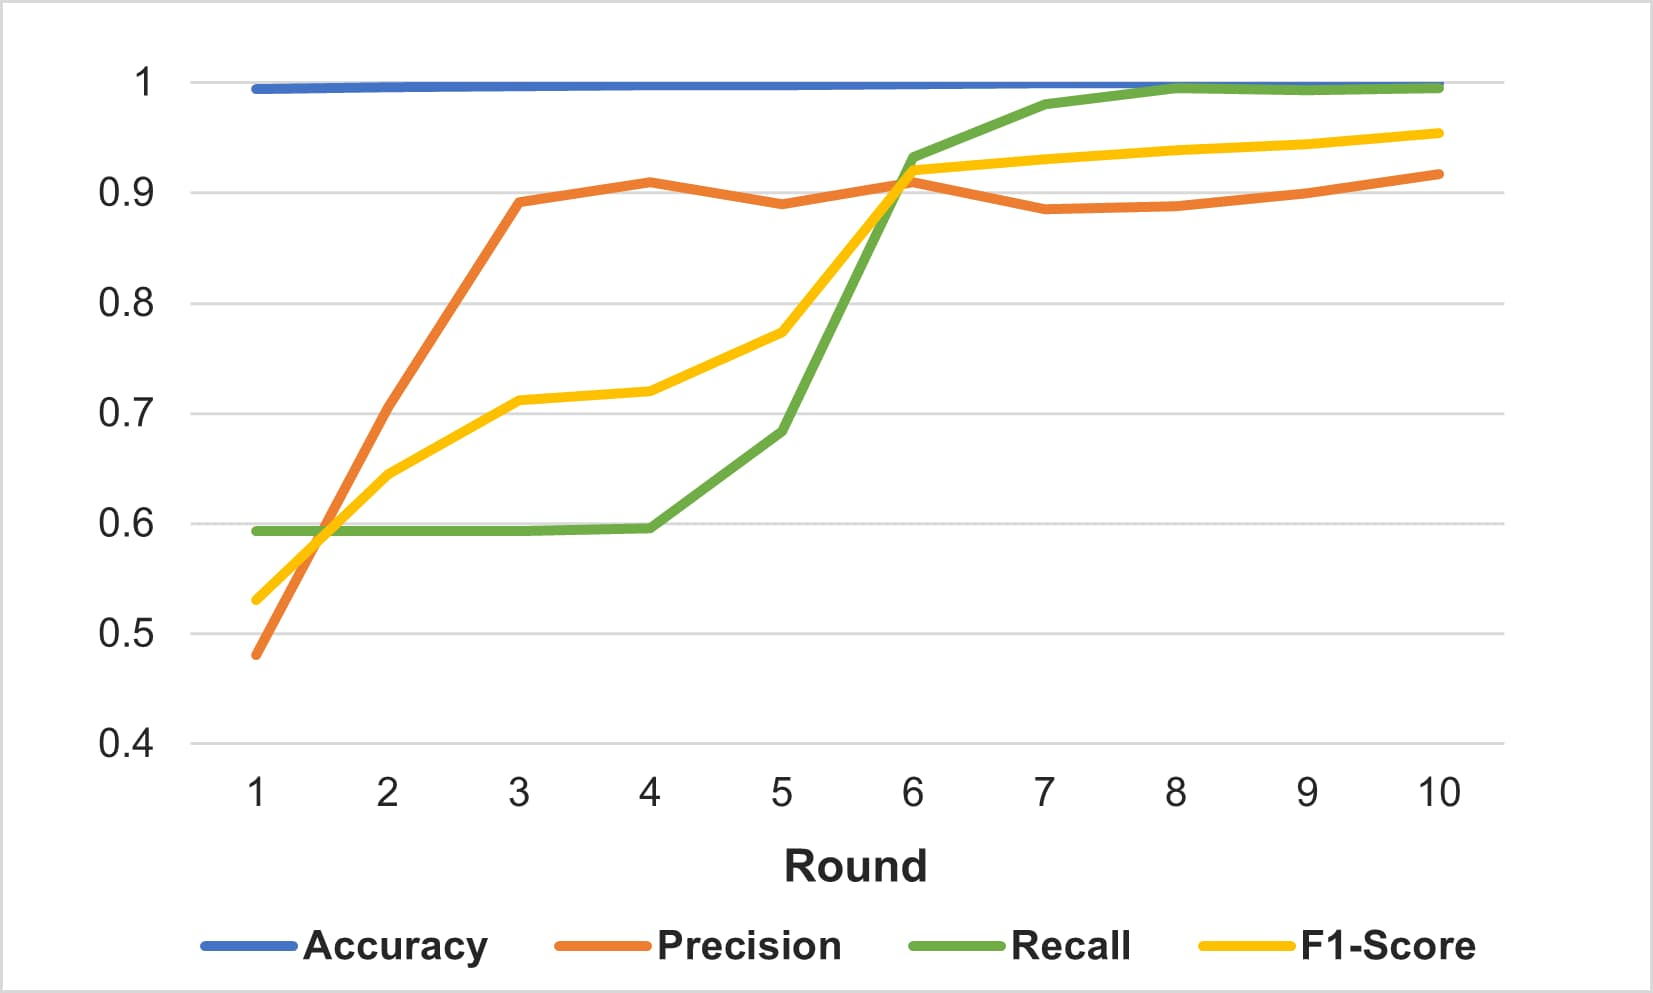
\includegraphics[width=0.5\linewidth]{src/images/chapter4/Node-GraphSAGE.jpg}\label{fig:node}}%
 \caption[Kết quả đánh giá khả năng hội tụ của mô hình TGraphSAGE]{Kết quả đánh giá khả năng hội tụ của mô hình TGraphSAGE trong trường hợp (A) sử dụng thuộc tính của nút và cạnh, và (B) chỉ sử dụng thuộc tính của nút}%
 \label{fig:node&edge-vs-edge}%
\end{figure}



\section{Diễn giải dự đoán của các mô hình IDS}
\subsection{Tiêu chí đánh giá các giải thích cho dự đoán đến từ các mô hình IDS}

Như đã đề cập trong \textit{Mục \ref{sec:interpretability-metric}}, chúng ta có thể đánh giá một giải thích có tốt hay không dựa vào một trong ba phương pháp: \textit{đánh giá ở mức độ ứng dụng}, \textit{đánh giá ở mức độ con người}, \textit{đánh giá ở mức độ chức năng}. Tuy nhiên, dữ liệu mà chúng ta dựa vào để phân tích giải thích là rất khó để có thể đánh giá bởi người dùng không có chuyên môn và các phương pháp được sử dụng để tạo giải thích như bộ khung SHAP và GNNExplainer nói riêng cũng như các phương pháp tạo giải thích cho các mô hình sâu huấn luyện nói chung là chưa tồn tại các công thức hay phương pháp toán học có thể đánh giá được khả năng diễn giải của các giải thích được tạo bởi các phương pháp trên. Vì vậy, chúng tôi sẽ thực hiện đánh giá giải thích thông qua phương pháp \textit{đánh giá ở mức độ ứng dụng}. Cụ thể, chúng tôi sẽ tiến hành phân tích các giải thích được tạo bởi các phương pháp tạo giải thích và sử dụng kiến thức chuyên môn của mình để đánh giá các giải thích dựa trên các dữ liệu đầu và cấu trúc của mô hình.
%Gilpin và các cộng sự \cite{gilpin2018explaining} đề xuất rằng một giải thích có thể được đánh giá dựa trên khả năng diễn giải (interpretability) và sự đầy đủ (completeness). Khả năng diễn giải là cách mà một giải thích mô tả các thành phần bên trong của một hệ thống một cách dễ hiểu đối với con người. Tiêu chí này thường liên quan đến nhận thức, kiến thức và định kiến của người sử dụng. Trong khi đó, sự đầy đủ cung cấp một mô tả chính xác về cách một hệ thống hoạt động nhưng thường gây khó khăn ngay cả đối với những chuyên gia trong trường hợp cần giải thích các chương trình máy tính như các mạng nơ-ron nhân tạo. Do sự khác biệt này trong mục tiêu, việc đạt được đồng thời khả năng diễn giải và sự đầy đủ là rất khó khăn. Do đó, trong các tình huống thực tế, chúng ta có thể chấp nhận một giải thích có khả năng diễn giải cao nhưng đổi lại là việc sự đầy đủ bị giảm đi.
%\bigbreak\noindent
%Gilpin và các cộng sự cũng đề xuất hai phương pháp đánh giá cho các giải thích được tạo bởi các phương pháp tập trung vào việc giải thích quá trình hoạt động của các mạng nơ-ron nhân tạo như bộ khung SHAP và GNNexplainer như sau: đánh giá sự đầy đủ so với mô hình gốc và đánh giá tính đầy đủ thông tác vụ thay thế. Hai phương thức trên tập trung vào việc kiểm tra độ chính xác của các mô hình thay thế cục bộ trọng việc giải thích một dự đoán nào đó. Tuy nhiên, nhiều nghiên cứu trước đó, bao gồm \cite{lundberg2017unified}, \cite{ribeiro2016should}, \cite{ ancona2017towards} và \cite{ying2019gnnexplainer}, đã chỉ ra rằng bộ khung SHAP và GNNexplainer là các phương pháp đã chứng minh được tính chính xác của các giải thích của mình thông qua hai phương pháp đề xuất trên. Do đó, chúng tôi quyết định chỉ kiểm tra khả năng diễn giải của các giải thích được tạo khung SHAP và GNNExplainer thông qua phương pháp đánh giá dựa trên con người ở mức độ ứng dụng như được đề cập ở \textbf{Mục \ref{sec:interpretability-metric}}. %, để phân tích khả diễn giải của các giải thích được tạo ra bởi bổ khung SHAP và GNNExplainer.% đặc biệt trong các trường hợp giải thích được kết hợp cho cả dự đoán đúng và sai từ quan điểm của một chuyên gia ngành.

\subsection{Diễn giải dự đoán của mô hình NIDS}

Bộ khung SHAP cung cấp nhiều chức năng trực quan hóa để giải thích các quyết định của mô hình bằng Shapley value. Chúng ta có thể giải thích một dự đoán thông qua hàm waterfall\footnote{\url{https://shap.readthedocs.io/en/latest/example_notebooks/api_examples/plots/waterfall.html}}, như được thể hiện trong \textbf{Hình \ref{fig:SHAP-waterfall}}. Trục hoành của hình được tạo bởi hàm waterfall mô tả giá trị dự đoán của mô hình. Trong khi đó, mỗi hàng đại diện cho đóng góp tích cực (màu đỏ) hoặc tiêu cực (màu xanh) của từng thuộc tính. Các đóng góp này sẽ di chuyển đầu ra của mô hình từ giá trị cơ sở (giá trị của $E[f(x)]$ tương đương với $\phi_0$ trong \textbf{Công thức \ref{eq:SHAP_explain_function}}) đến giá trị đầu ra cuối cùng (giá trị của $f(x)$).

\begin{figure}[h]
\centering
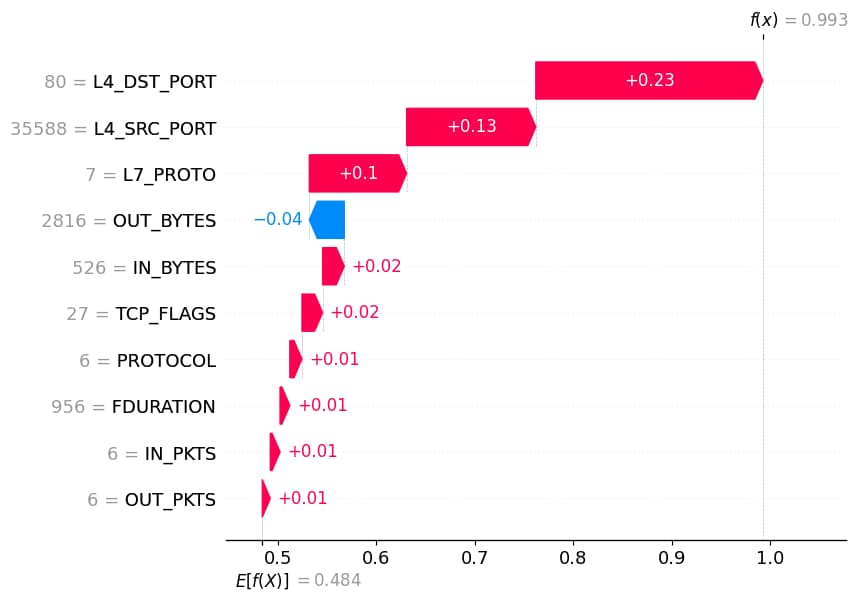
\includegraphics[width=\textwidth]{src/images/chapter4/SHAP-waterfall.jpg}
\caption{Giải thích cho một dự đoán từ mô hình GRU\&CNN}
\label{fig:SHAP-waterfall}
\end{figure}

\bigbreak\noindent
Từ \textbf{Hình \ref{fig:SHAP-waterfall}}, ta có thể thấy rõ ràng rằng mô hình GRU\&CNN phân loại \textit{flow} đầu vào là độc hại với số điểm gần như tuyệt đối là 0.993 và L4\_DST\_PORT là thuộc tính có đóng góp lớn nhất trong dự đoán trên (0.23). Ba đặc trưng có ảnh hưởng lớn nhất tiếp theo sau đặc trưng L4\_DST\_PORT đều có tác động tích cực trong việc xây dựng quyết định \textit{flow} đầu vào là độc hại. Trong khi thuộc tính OUT\_BYTES có tác động tiêu cực nhưng không ảnh hưởng quá nhiều đến dự đoán và các thuộc tính còn lại không có hoặc có tác động rất nhỏ đến quyết định của mô hình. Tuy nhiên, mặc dù mô hình đã đưa ra dự đoán rất tự tin cho thấy rằng \textit{flow} đầu vào là độc hại nhưng giải thích cho thấy rằng dự đoán này phụ thuộc mạnh mẽ vào các đặc trưng L4\_DST\_PORT và L4\_SRC\_PORT. Trong khi, dựa trên kiến thức chuyên môn của chúng tôi, các thuộc tính này thường ít quan trọng trong việc phát hiện các cuộc tấn công mạng trong các kịch bản thực tế. Điều này cho thấy rằng mô hình có thể đã bị ràng buộc quá chặt với ngữ cảnh của tập dữ liệu và đưa ra đánh giá một \textit{flow} là độc hại dựa trên một số giá trị nhất định của thuộc L4\_DST\_PORT và L4\_SRC\_PORT.

\bigbreak\noindent
Thay vì chỉ giải thích cho một dự đoán, chúng tôi thực hiện giải thích một tập các dự đoán khác nhau và tổng hợp chúng thông qua mô hình GRU\&CNN thông qua hàm beeswarm\footnote{\url{https://shap.readthedocs.io/en/latest/example_notebooks/api_examples/plots/beeswarm.html}} để có cái nhìn tổng quan hơn về tác động của các thuộc tính đối với dự đoán của mô hình. Hơn thế nữa, thay vì giải thích các mẫu ngẫu nhiên như các nghiên cứu liên quan \cite{wang2020explainable} và \cite{9825734}, chúng tôi thực hiện giải thích 4 tập dữ liệu riêng biệt dựa trên kết quả đầu ra của chúng (TP, FP, TN, FN). Cụ thể hơn, chúng tôi trích xuất các tập dữ liệu này từ dự đoán của mô hình GRU\&CNN trên dữ liệu kiểm tra với mỗi tập bao gồm 100 mẫu. Sau đó, đưa các tập dữ liệu này vào hàm beeswarm và tổng hợp chúng như trong \textbf{Hình \ref{fig:TP-TN-FN-FP}}. 

\begin{figure}[h]%
 \centering
 \subfloat[Tổng hợp cho các giải thích cho các dự đoán TP]{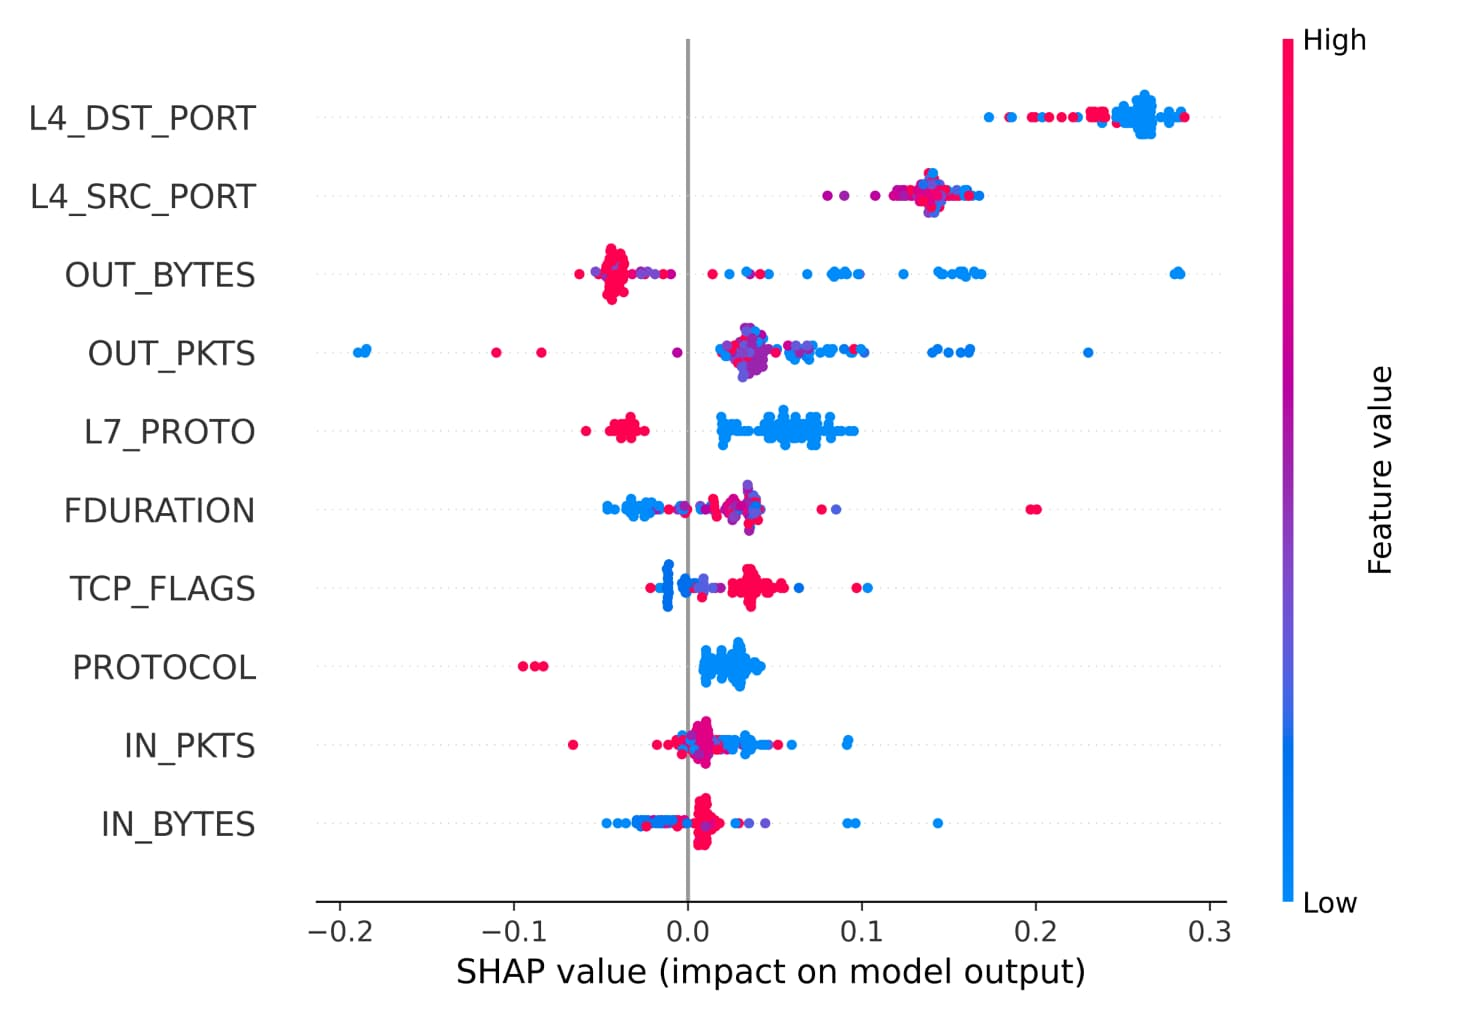
\includegraphics[width=0.5\linewidth]{src/images/chapter4/TP.jpg}\label{fig:TP}}%
 \subfloat[Tổng hợp cho các giải thích cho các dự đoán TN]{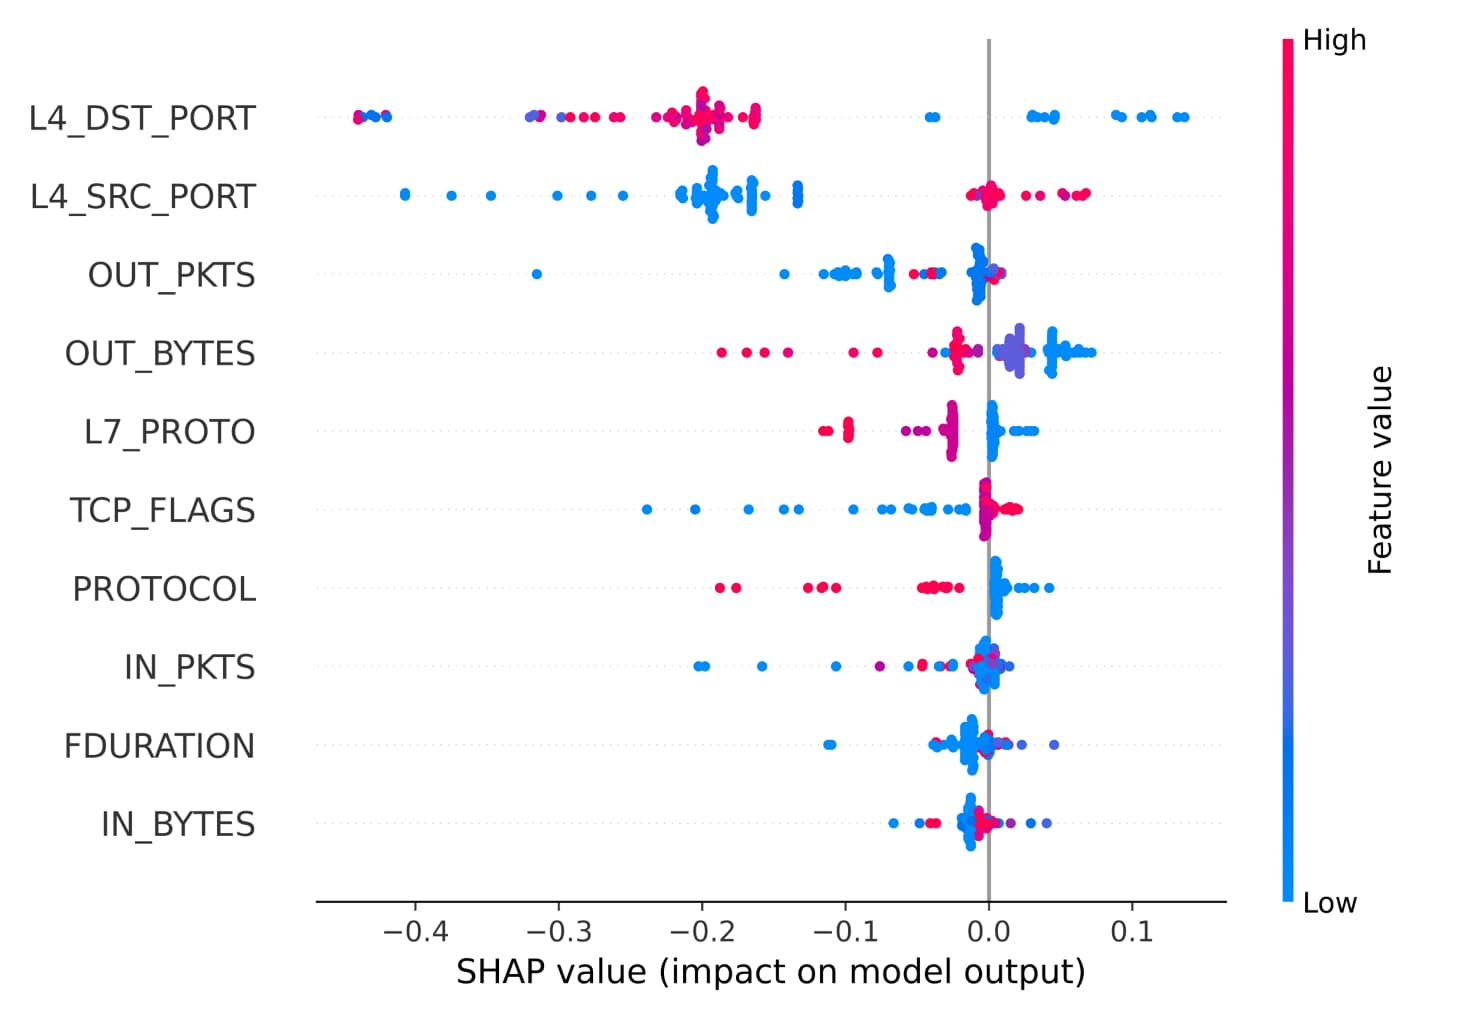
\includegraphics[width=0.5\linewidth]{src/images/chapter4/TN.jpg}\label{fig:TN}}\\
 \subfloat[Tổng hợp cho các giải thích cho các dự đoán FN]{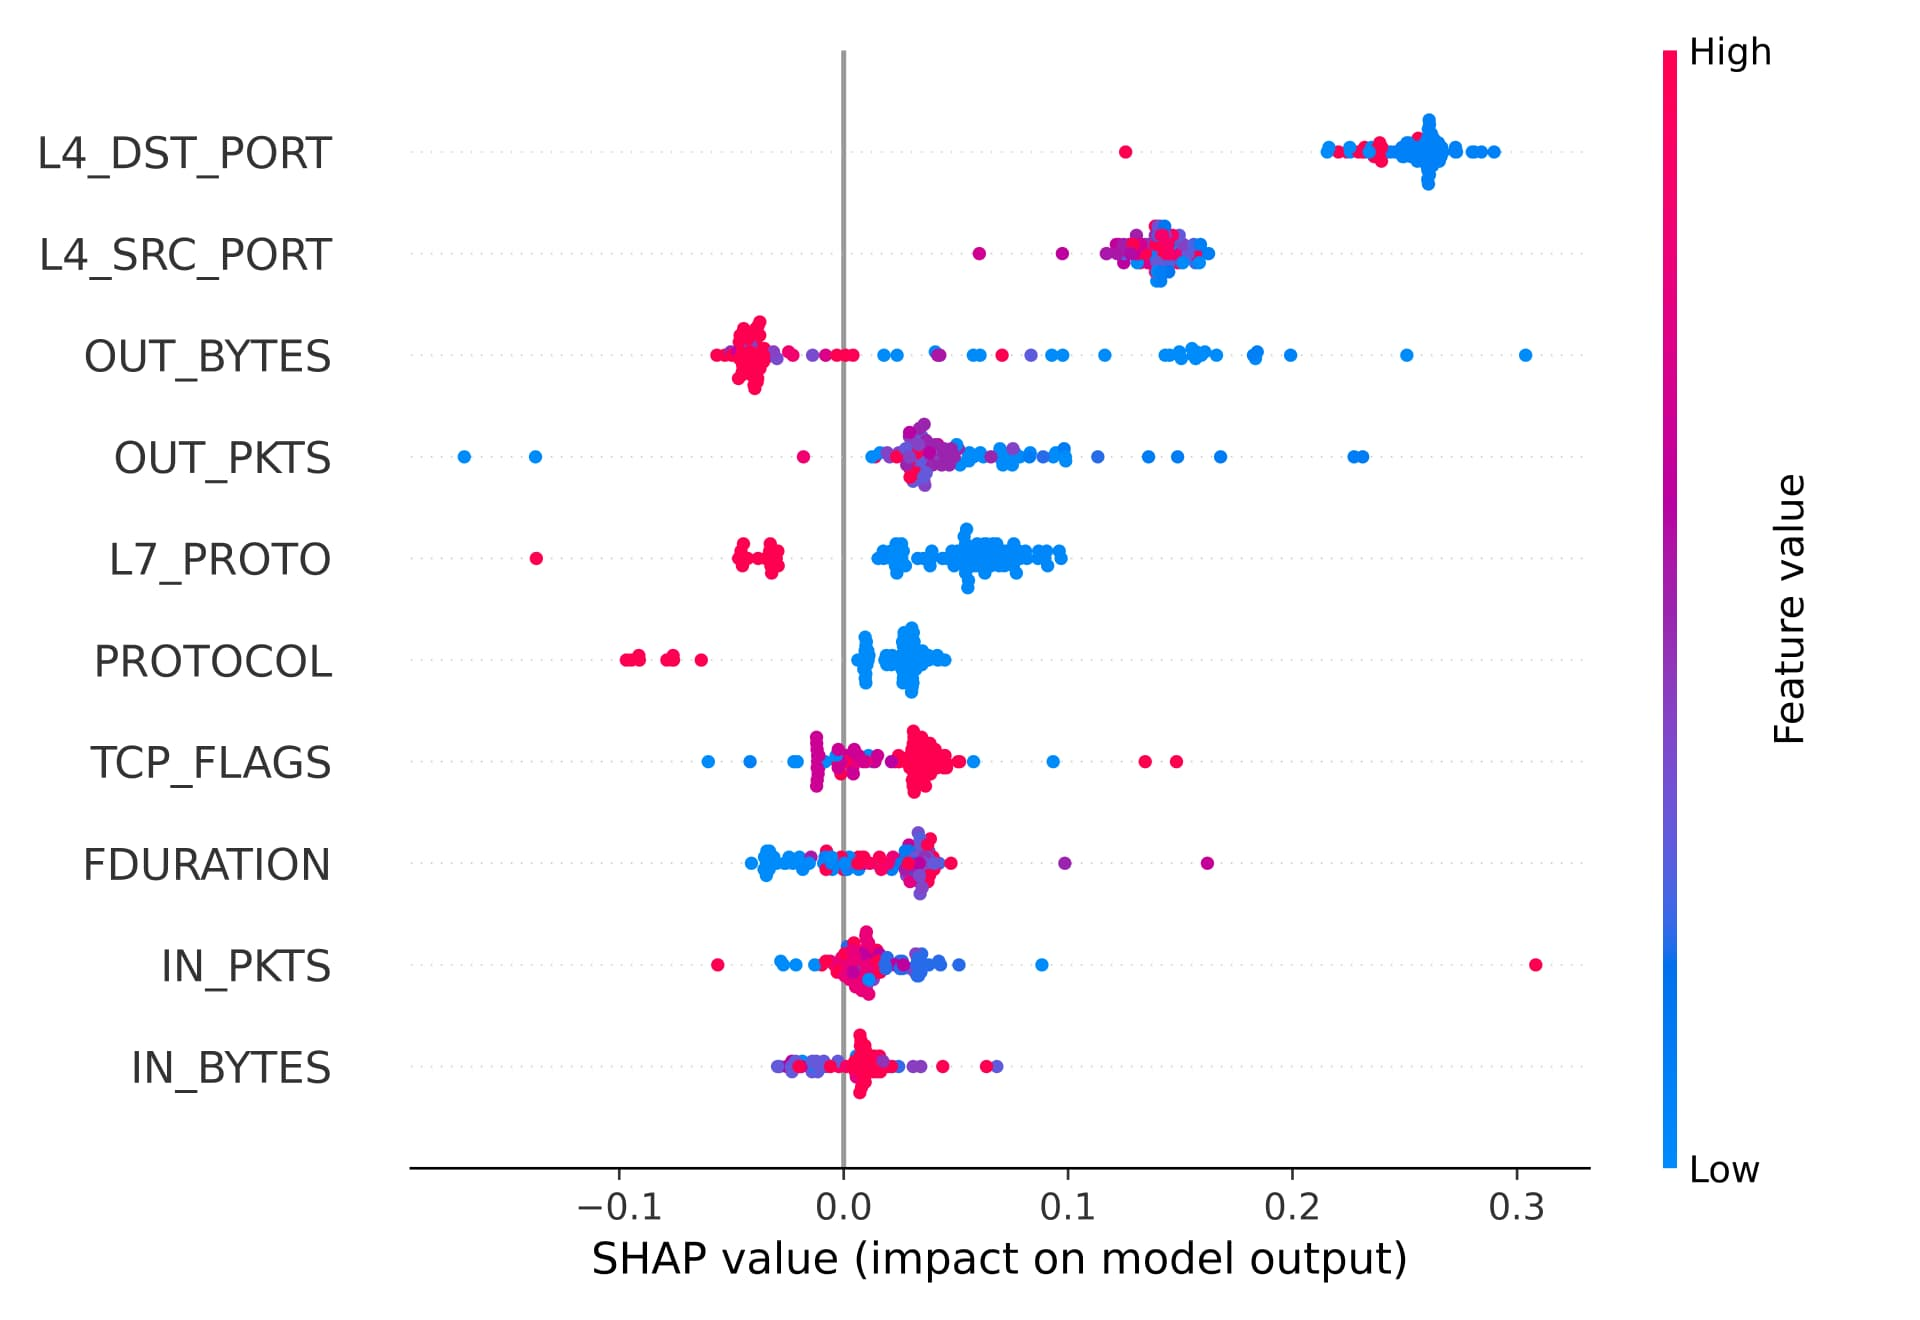
\includegraphics[width=0.5\linewidth]{src/images/chapter4/FN.jpg}\label{fig:FN}}%
 \subfloat[Tổng hợp cho các giải thích cho các dự đoán FP]{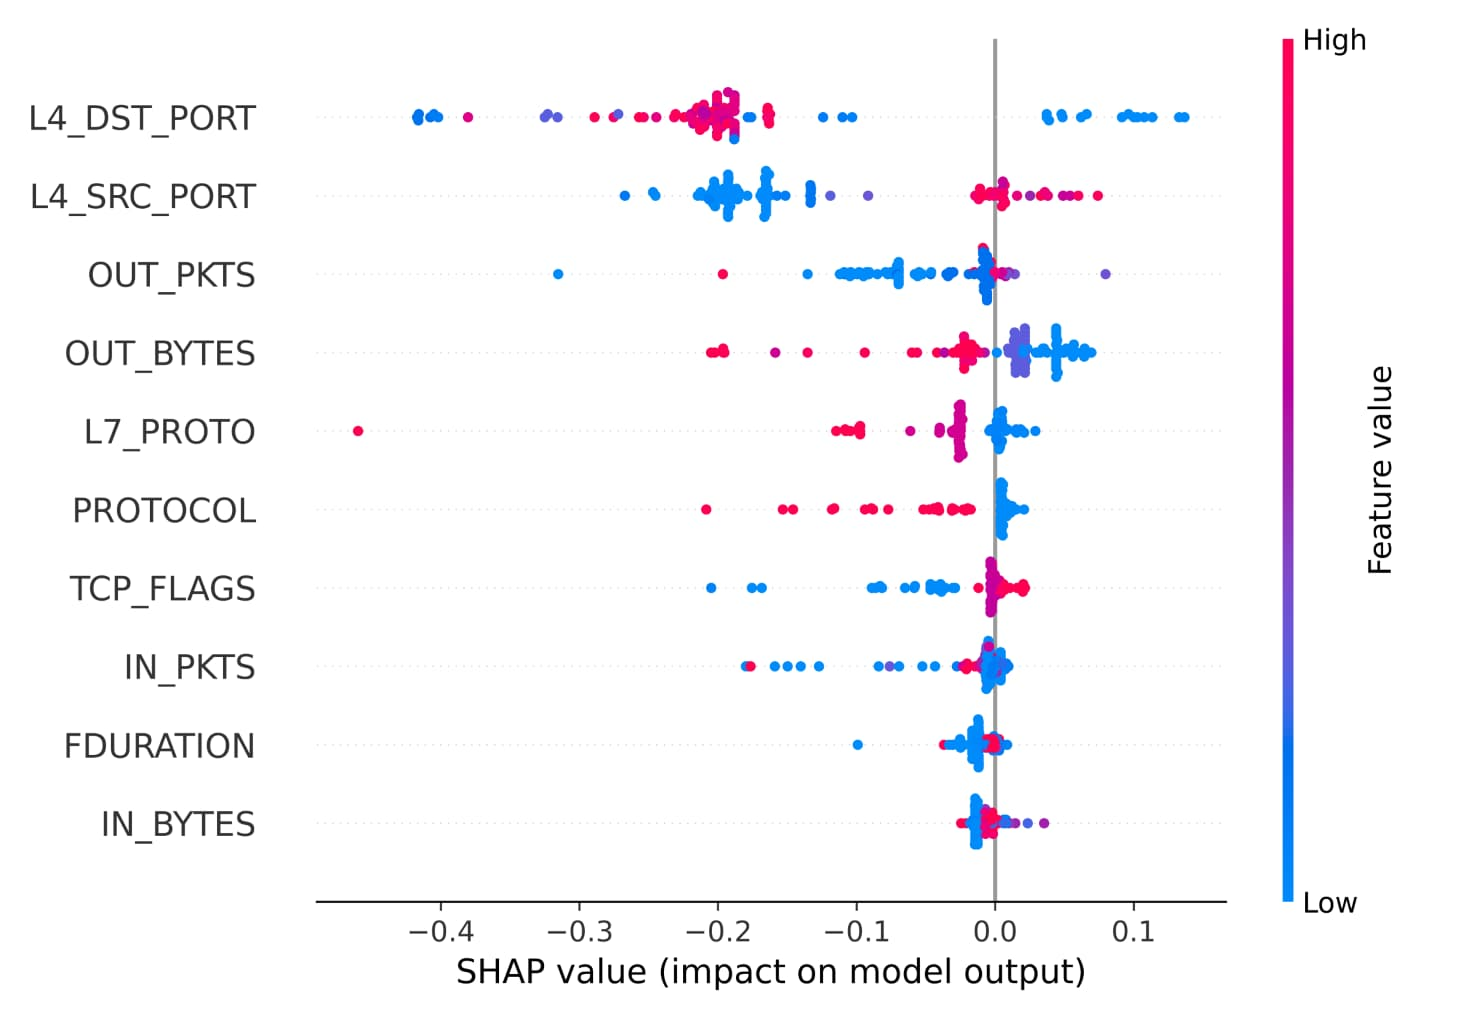
\includegraphics[width=0.5\linewidth]{src/images/chapter4/FP.jpg}\label{fig:FP}}%
 \caption[Tổng hợp các giải thích cho các dự đoán từ mô hình GRU\&CNN]{Tổng hợp các giải thích cho các dự đoán từ mô hình GRU\&CNN dựa trên lớp của chúng (TP, TN, FN, FP)}%
 \label{fig:TP-TN-FN-FP}%
\end{figure}

\bigbreak\noindent
\textbf{Hình \ref{fig:TP}} và \textbf{Hình \ref{fig:TN}} trình bày các giải thích cho 100 dự đoán TP và 100 dự đoán TN được tạo bởi mô hình GRU\&CNN. Mặc dù cả hai biểu đồ đều cho kết quả gần như giống nhau cho năm thuộc tính có ảnh hưởng lớn nhất nhưng cũng có một số khác biệt quan trọng. Kết quả trong \textbf{Hình \ref{fig:TP}} cho thấy thuộc tính có ảnh hưởng lớn nhất (L4\_DST\_PORT) có một tác động tích cực và nhất quán đến dự đoán của mô hình với các giá trị đóng góp dao động từ 0.15 đến 0.3. Giá trị thực tế của thuộc tính này trong hầu hết các mẫu nằm trong khoảng giá trị thấp. Trong khi đó, đóng góp của đặc trưng L4\_DST\_PORT trong \textbf{Hình \ref{fig:TN}} dao động từ -0.4 đến 0.1. Đáng chú ý, hầu hết các mẫu có giá trị cao cho thuộc tính này thể hiện một đóng góp trong khoảng từ -0.3 đến -0.2. Điều này cho thấy rằng các giá trị trong khoảng này có ảnh hưởng tiêu cực đáng kể đến dự đoán của mô hình và làm cho các mẫu này có khả năng là độc hại. Tuy nhiên, một số mẫu có giá trị thấp cho thuộc tính có sự đóng góp rất cao. Điều này có thể một quyết định không chắc chắn của mô hình hoặc một quyết định đã bị ràng buộc với một port cụ thể (trường hợp mà đóng góp có tác động lên đến -0.4). Từ phân tích trên, ta có thể thấy rằng đóng góp của đặc trưng L4\_DST\_PORT cho các dự đoán TP luôn có tác động tích cực và hội tụ trong một khoảng giá trị nhất định, trong khi đóng góp của thuộc tính L4\_DST\_PORT cho các dự đoán TN cũng hội tụ trong một khoảng giá trị nhất định nhưng có một số giá trị không mong đợi do ảnh hưởng của các mẫu có giá trị thấp trong các thuộc tính này.
\bigbreak\noindent
Tương tự, trong \textbf{Hình \ref{fig:TP}}, đóng góp của thuộc tính L4\_SRC\_PORT trong 100 dự đoán TP có các đặc điểm tương tự như đặc trưng L4\_DST\_PORT nhưng hội tụ trong khoảng đóng góp thấp hơn và giá trị của thuộc tính này được phân phối trong một khoảng rộng hơn. Ngoài ra, đóng góp của thuộc tính L4\_SRC\_PORT trong \textbf{Hình \ref{fig:TP}} cũng có sự tương đồng với thuộc tính quan trọng nhất nhưng đóng góp của thuộc tính này lại hội tụ ở điểm thấp hơn và giá trị của thuộc tính có xu hướng ngược lại so với đặc trưng quan trọng nhất. Hai thuộc tính có độ quan trọng cao tiếp theo trong \textbf{Hình \ref{fig:TP}} và \textbf{Hình \ref{fig:TN}} là hai thuộc tính duy nhất có vị trí khác nhau trong năm thuộc tính có ảnh hưởng lớn nhất. Thuộc tính OUT\_BYTES có đóng góp tiêu cực đến dự đoán cho các mẫu có giá trị cao trong thuộc tính này và đóng góp tích cực đến các mẫu có giá trị thấp. Tuy nhiên, đối với các dự đoán TP, đóng góp của OUT\_BYTES hội tụ mạnh mẽ với các mẫu có giá trị cao của đặc trưng này, trong khi đối với dự đoán TN, đóng góp hội tụ với các mẫu có giá trị thấp và trung bình. Hơn thế nữa, mặc dù các mẫu TP và TN có giá trị thấp trong đặc trưng OUT\_PKT, đóng góp cho đặc trưng này có tác động ngược nhau trong mỗi trường hợp: tác động tích cực đối với dự đoán TP và tác động tiêu cực đối với dự đoán TN. Tương tự, chúng ta có thể phân tích các đặc trưng còn lại để khám phá mối quan hệ giữa dự đoán TP và TN và cung cấp thông tin về cách mỗi đặc trưng ảnh hưởng đến quyết định của mô hình.
\bigbreak\noindent
Tuy nhiên, những mẫu FN và mẫu FP cũng có các giải thích với các mẫu TP và mẫu TN, như được hiển thị trong \textbf{Hình \ref{fig:FN}} và \textbf{Hình \ref{fig:FP}}. Điều này cho thấy rằng các mẫu độc hại có phân phối dữ liệu tương tự với các mẫu không độc hại và các mẫu này có thể làm cho mô hình bị nhầm lẫn và phân loại sai chúng. Từ hiểu biết của chúng tôi, những sự nhầm lẫn này là có thể được lý giải khi áp dụng vào một kịch bản thực tế. Với các trường hợp tấn công DoS,  cuộc tấn công DoS xảy ra khi có một lưu lượng mạng lớn vượt quá một hạn mức nào đó di chuyển trong hệ thống. Do đó, việc xác định xem có xảy ra cuộc tấn công hay không phụ thuộc vào lượng lưu lượng và hệ thống cụ thể. Tuy nhiên, giống như hầu hết các nghiên cứu khác, chúng tôi phân loại dự đoán của mô hình là độc hại nếu nó vượt quá một ngưỡng xác định (thông thường là 0.5) và ngưỡng này có thể không phải là ngưỡng đo chính xác trong tất cả các trường hợp. Bên cạnh những nguyên nhân trên, sự nhầm lẫn này cũng có thể cho thấy việc gán nhãn sai trong tập dữ liệu thực nghiệm hoặc thậm chí là một tín hiệu cho một cuộc tấn công đối kháng.


\subsection{Diễn giải dự đoán của mô hình PIDS}

Chúng tôi trực quan hóa giải thích của GNNExplainer cho dự đoán của mô hình PIDS như trong \textbf{Hình \ref{fig:explained_benign}} và \textbf{Hình \ref{fig:explained_malicious}}. Trong các giải thích được trực quan hóa trên, nút trung tâm (nút màu xanh lá cây) là nút mà dự đoán của nó sẽ được giải thích. Các nút hàng xóm trong khoảng k-hop xung quanh nút được giải thích được hiển thị với dự đoán của chúng và các cạnh gán bằng độ quan trọng của chúng được tạo bởi GNNExplainer. Các giá trị biểu thị độ quan trọng này có giá trị nằm trong khoảng $[0, 1]$ và bằng cách đặt ngưỡng giá trị là 0.5, chúng tôi xác định các đường đi quan trọng để truyền và tổng hợp thông tin. Các đường quan trọng đó là các cạnh màu xanh dương với giá trị thể hiện độ quan trọng của cạnh lớn hơn ngưỡng đặt ra và cạnh màu xám không quan trọng, có điểm quan trọng bé hơn ngưỡng đặt ra. Sự thay đổi màu từ xanh nhạt sang xanh đậm và độ dày của cạnh thể hiện sự gia tăng trong độ quan trọng của các cạnh.
\bigbreak\noindent
\textbf{Hình \ref{fig:explained_benign}} hiển thị kết quả giải thích của một nút lành tính. Ngoại trừ hai nút ở phía dưới, các nút lân cận còn lại đều thể hiện độ quan trọng của chúng với giá trị lớn hơn 0.6 đối với dự đoán của nút được phân tích. Để hiểu rõ điều gì khiến khiến cho các cạnh đó trở nên quan trọng với dự đoán, chúng tôi đã tiến hành phân tích các giá trị ban đầu của các nút. Tất cả các kết nối đơn lẻ xung quanh nút được dự đoán đều có giá trị là ``\emph{A subject object has the subtype named process, and it modified a process using sshd.}". Lý do giải thích không quan tâm đến hai nút ở phía dưới là bởi mục tiêu của GNNExplainer là tạo ra một đồ thị con tối thiểu nên nó sẽ loại bỏ các cạnh (gán cho chúng độ quan trọng thấp) nếu việc loại bỏ chúng không làm biến đổi dự đoán của PIDS. Ngoài ra, giá trị của nút trung tâm là ``\emph{A file object has the subtype named file, and it was modified using find, ...}" và nút lận cận có số cạnh kết nối lớn nhất với nút được dự đoán có giá trị là ``\emph{A subject object has the subtype named process, and it modified a process using find, ...}". Và theo kinh nghiệm của chúng tôi, những giá trị ban đầu này đều là hành vi không gây hại cho nên chúng ta có thể kết luận rằng nút trung tâm được phân loại đúng bởi mô hình PIDS là một nút không gây hại.

\begin{figure}[h]
    \centering
    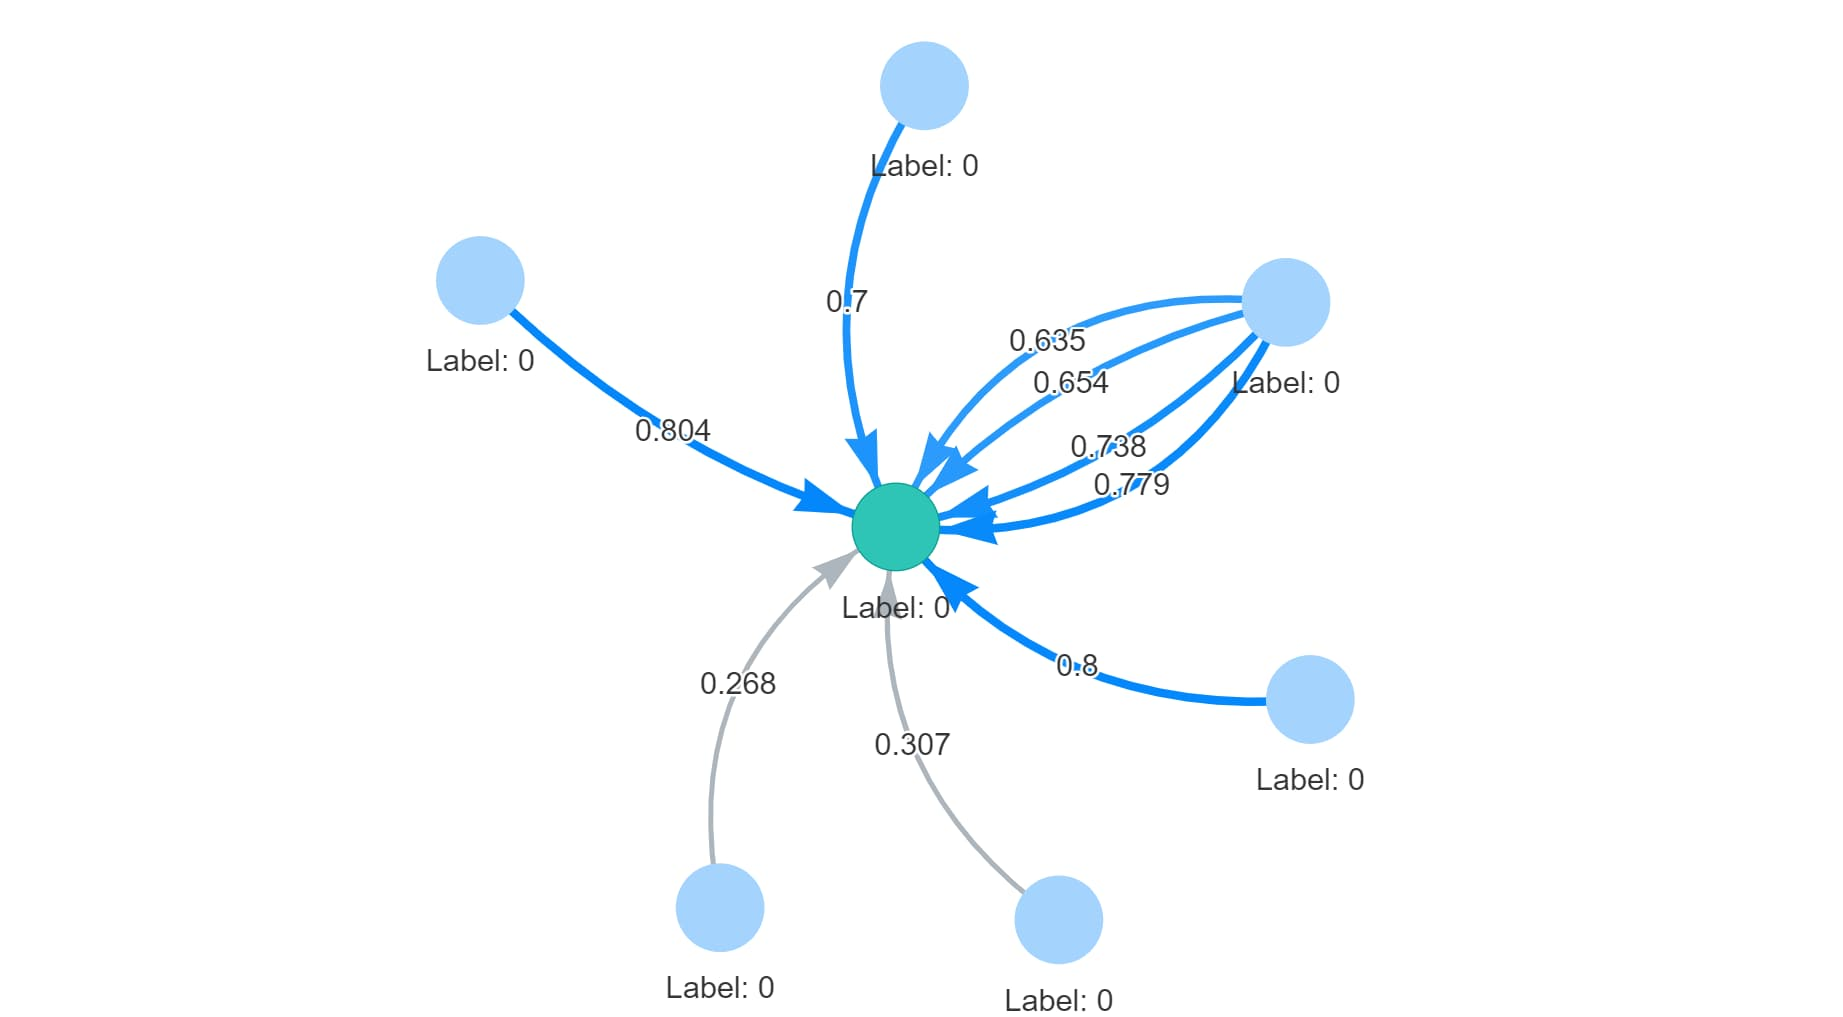
\includegraphics[width=\textwidth]{src/images/chapter4/explained-benign.jpg}
    \caption{Giải thích cho dự đoán từ mô hình TGraphSAGE cho một nút lành tính}
    \label{fig:explained_benign}
\end{figure}
\bigbreak\noindent
\textbf{Hình \ref{fig:explained_malicious}} hiển thị kết quả giải thích của một nút độc hại. Từ hình vẽ, ta có thể thấy được rằng các nút xung quanh nút được dự đoán đều được dự đoán là độc hại. Điều đó chứng tỏ mô hình PIDS có khả năng gom nhóm được chuỗi các sự kiện độc hại và cũng chứng tỏ rằng các nút độc hại xung quanh có ảnh hưởng đến kết quả dự đoán của một nút. Khi xem xét các giá trị ban đầu của nút được dự đoán, ta thấy rằng nút này chứa các tệp tin mà chúng tôi biết được đây là những tệp tin được đánh dấu là độc hại trong thí nghiệm DARPA TCE3, các tệp tin độc hại có thể kể đến như: ``\emph{/var/log/sendmail}", ``\emph{/tmp/font}" và ``\emph{/tmp/minions}". Từ đó, ta có thể kết luận nút được dự đoán được phân loại đúng bởi mô hình PIDS là một nút độc hại.

\begin{figure}[h]
    \centering
    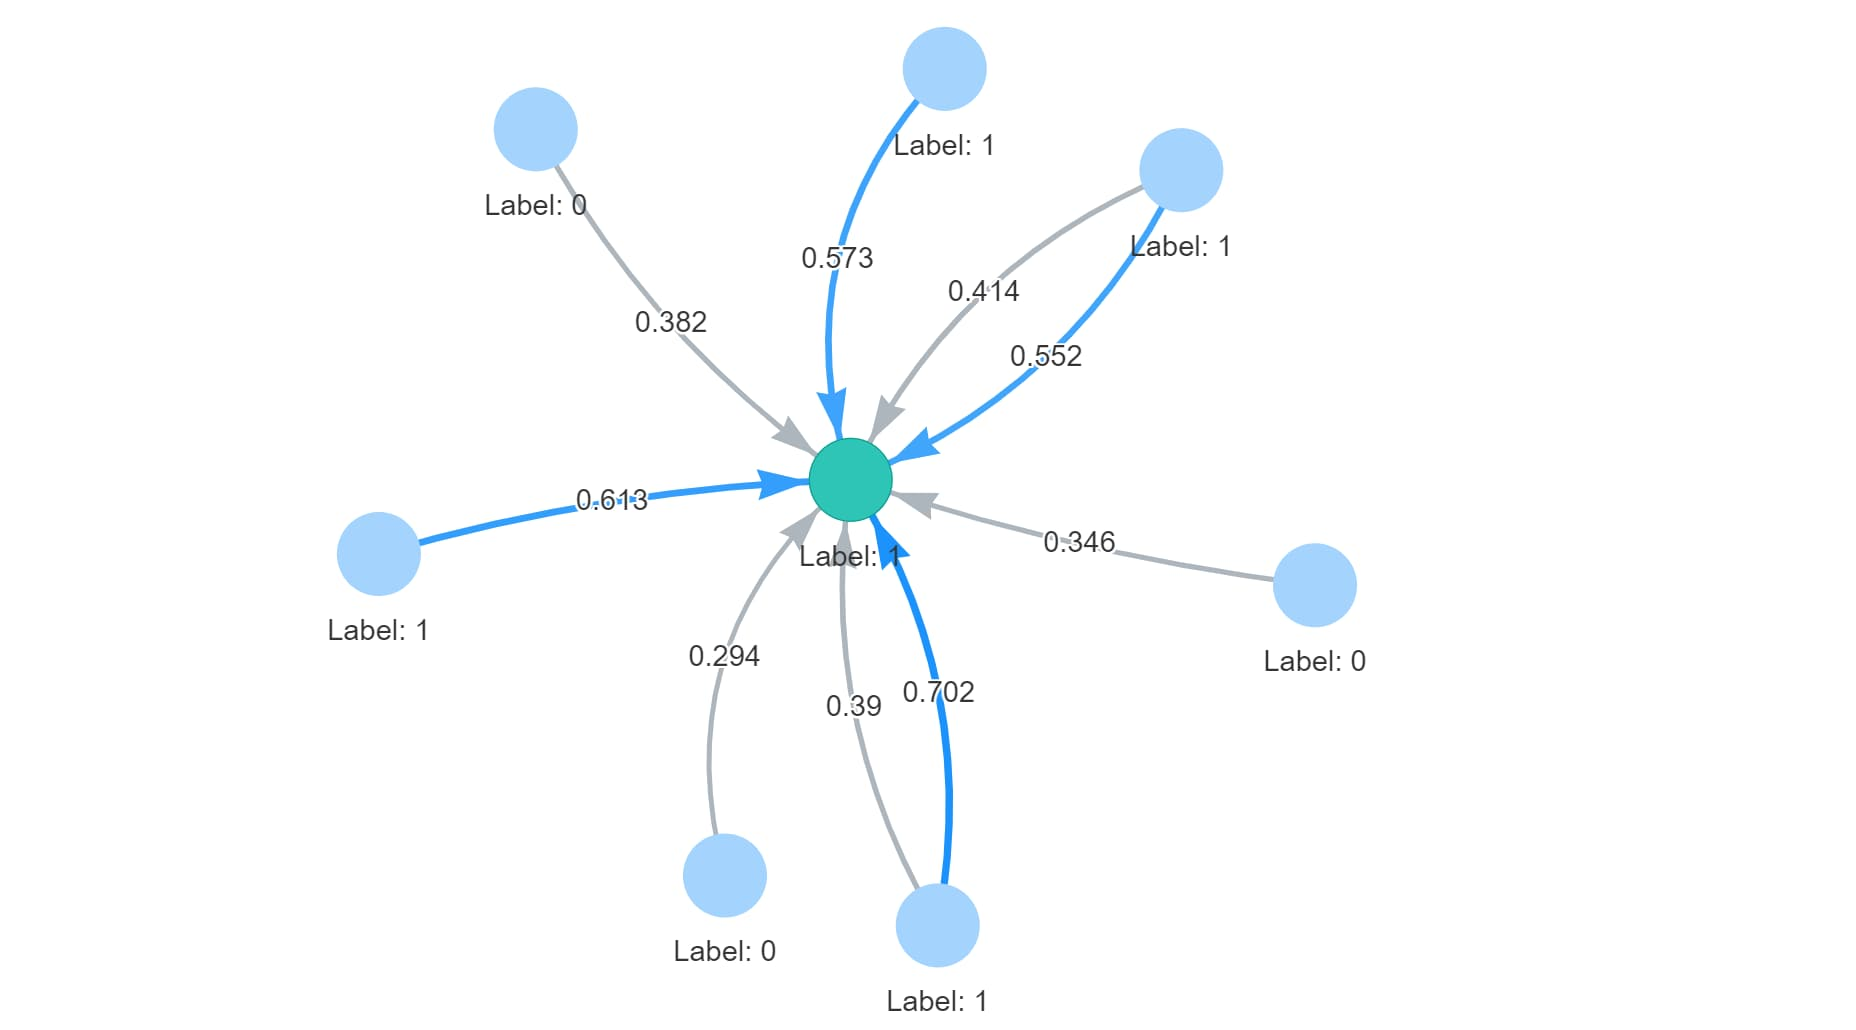
\includegraphics[width=\textwidth]{src/images/chapter4/explained-malicious.jpg}
    \caption{Giải thích cho dự đoán từ mô hình TGraphSAGE cho một nút độc hại}
    \label{fig:explained_malicious}
\end{figure}

\subsection{Đánh giá phương pháp xác định độ tin cậy của các dự đoán từ các mô hình IDS}

Từ các tập dữ liệu kiểm tra được sử dụng để đánh giá hai mô hình IDS trong \textbf{Mục \ref{sec:implemented-FL-based-IDS}}, chúng tôi trước tiên tạo ra một tập dữ liệu dựa trên đầu ra của lớp áp chót với kích thước là 400 được chia đều thành bốn lớp (TP, TN, FP, FN), như mô tả trong \textbf{Thuật toán \ref{alg:proposed-methodology}}. Chúng tôi cũng sử dụng một kỹ thuật được gọi là t-SNE \cite{van2008visualizing} để trực quan hóa và so sánh tập dữ liệu gốc với tập dữ liệu dựa trên đầu ra của lớp áp chót được tạo bởi mô hình GRU\&CNN, như được hiển thị trong \textbf{Hình \ref{fig:compare-original-penultimate}}. Kỹ thuật trên được sử dụng để chứng minh rằng các giá trị đầu ra của lớp áp chót có thể dễ dàng sử dụng trong việc phân loại các dự đoán hơn so với dữ liệu gốc.

\begin{figure}[h]
\centering
 \subfloat[]{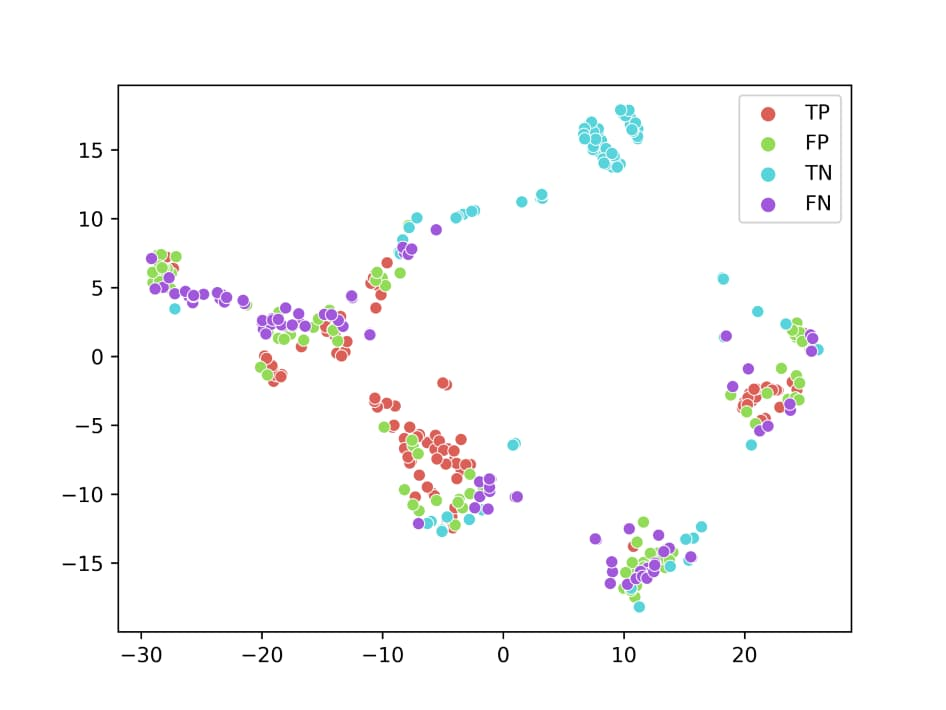
\includegraphics[width=0.5\linewidth]{src/images/chapter4/rawdata-tsne.jpg}\label{fig:rawdata-tsne}}%
 \subfloat[]{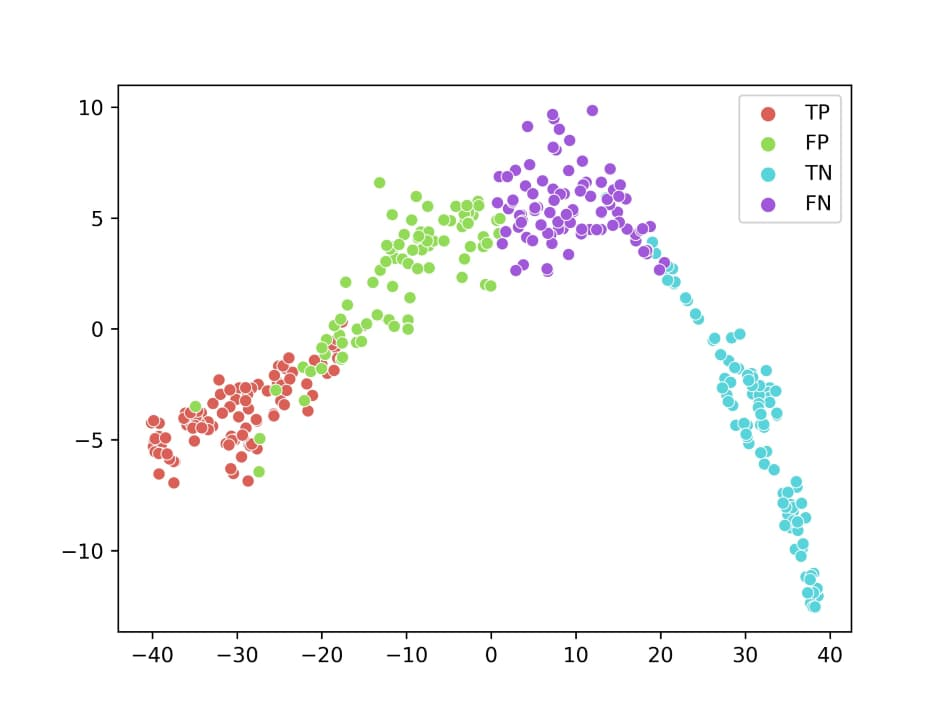
\includegraphics[width=0.5\linewidth]{src/images/chapter4/nep-tsne.jpg}\label{fig:nep-tsne}}%
\caption[Trực quan hóa dữ liệu với t-SNE]{Trực quan hóa bằng t-SNE cho (A) tập dữ liệu gốc và (B) tập dữ liệu dựa trên đầu ra của lớp áp chót}
\label{fig:compare-original-penultimate}
\end{figure}

\bigbreak\noindent
Từ \textbf{Hình \ref{fig:compare-original-penultimate}}, ta có thể thấy rằng dữ liệu dựa trên đầu ra của lớp áp chót được nhóm tốt hơn trong tập dữ liệu gốc, mặc dù có một số điểm dữ liệu dựa trong tập dữ liệu dựa trên đầu ra của lớp áp chót được đặt trong lớp sai. Bằng chứng này cho thấy việc kiểm tra chất lượng dự đoán trên đầu ra của lớp áp chót sẽ mang lại hiệu suất cao hơn so với dữ liệu gốc.
\bigbreak\noindent
Đối với bộ phân loại được sử dụng để xác định độ tin cậy của dự đoán, chúng tôi đơn giản là thực hiện tính trung bình khoảng cách giữa các mẫu được xem xét và các mẫu trong tập dữ liệu chuẩn bị trước. Sau đó, dự đoán được xem xét được gán vào lớp có trung bình khoảng cách nhỏ nhất. Chúng tôi chọn sử dụng phương pháp tính trung bình khoảng cách trong bộ phân loại của mình do thiếu mẫu cho các lớp FP và FN trong tập dữ liệu kiểm tra, mặc dù ở đó có rất nhiều mẫu cho các lớp TP và TN. Đặc biệt đối với mô hình GRU\&CNN, chúng tôi chỉ có 300 mẫu cho lớp FP và 183 mẫu cho lớp FN trong dữ liệu kiểm tra của chúng tôi. Để duy trì cân bằng giữa các lớp, chúng tôi quyết định tạo ra một tập dữ liệu huấn luyện gồm 400 mẫu và một tập dữ liệu kiểm tra gồm 360 mẫu với các mẫu trong các tập dữ liệu này được chia đều cho mỗi lớp. Sự thiếu hụt mẫu FP và FN còn trầm trọng hơn đối với mô hình GraphSAGE, trong đó, không có mẫu FN nào được tạo ra vì mô hình của chúng tôi luôn đạt recall bằng 1.0. Vì vậy chúng tôi chỉ có một tập dữ liệu huấn luyện với kích thước 120 mẫu (60 mẫu TP, 30 mẫu FP, 60 mẫu TN và 0 mẫu FN) và một tập dữ liệu kiểm tra gồm 80 mẫu (30 mẫu TP, 20 mẫu FP, 30 mẫu TN và 0 mẫu FN). Do kích thước nhỏ của các tập dữ liệu được tạo ra, chúng tôi không nên sử dụng những phương pháp quá phức tạp, gây ra tính toán không cần thiết và làm giảm hiệu suất phân loại. Mặc cho các hạn chế đã đề cập, phương pháp của chúng tôi vẫn đạt được độ chính xác ấn tượng xấp xỉ 0.9188 trong trường hợp của mô hình GRU\&CNN và 0.9875 trong mô hình TGraphSAGE.

\section{Hiện thực mô hình săn tìm tấn công APT trên từng zone}

Mục tiêu của chúng tôi là có thể mô phỏng một môi trường hoàn thiện, sát với mô hình đề ra nhất sử dụng các công cụ ảo hoá và giả lập. Chúng tôi ưu tiên những công cụ mã nguồn mở, những công cụ này hoàn toàn miễn phí, dễ dàng triển khai cũng như không phụ thuộc vào một bên nào cả. \textbf{Hình \ref{fig:APT-hunting-zone-with-tech}} mô tả một hệ thống săn tìm tấn công APT được triển khai trên một zone.

\begin{figure}[h]
    \centering
    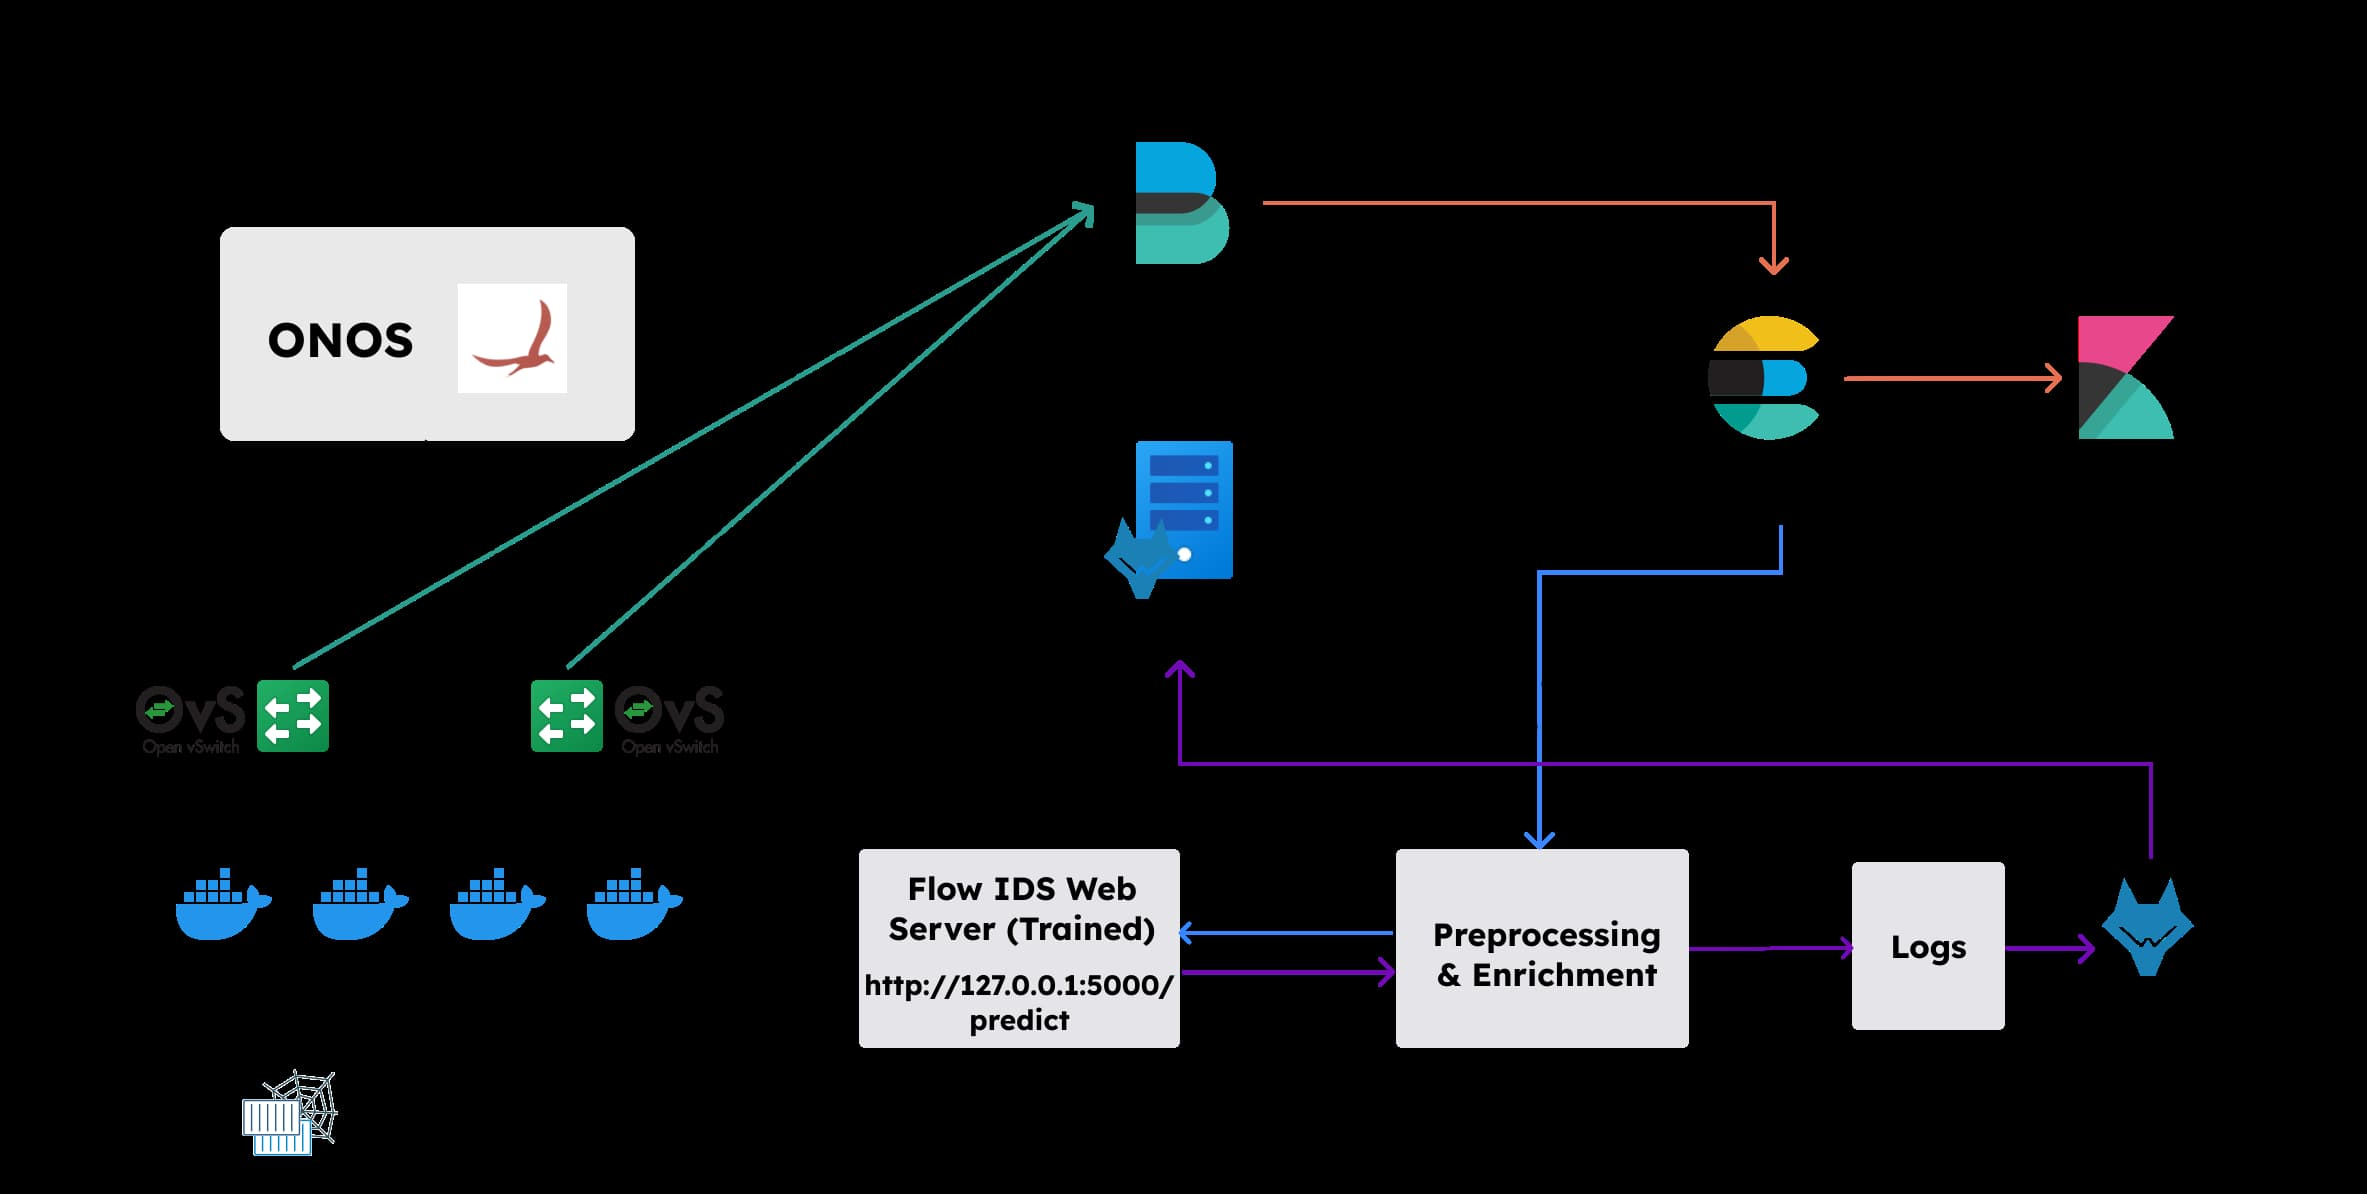
\includegraphics[width=\textwidth]{src/images/chapter4/threat-hunting-proprosed-model-with-tech.jpg}
    \caption{Mô hình săn tìm tấn công APT được triển khai cho một zone}
    \label{fig:APT-hunting-zone-with-tech}
\end{figure}


\subsection{Mạng SDN}

Nhằm xây dựng một hệ thống mạng ổn định và dễ theo dõi, chúng tôi quyết định thực hiện giả lập sử dụng \textit{Containernet} \footnote{Containernet: \url{https://containernet.github.io}}. Đây là một công cụ giả lập hệ thống mạng cùng với sử dụng các \textit{Docker} \footnote{Docker: \url{https://www.docker.com}} container như là các máy trong mạng. Bên cạnh đó, chúng tôi sử dụng \textit{ONOS} \footnote{ONOS: \url{https://opennetworking.org/onos/}}, là một trung tâm điều khiển mã nguồn mở được sử dụng rộng rãi, nhiều tính năng và kết hợp tốt với nhiều loại hệ thống mạng. Các switch trong mạng được cấu hình sử dụng OpenFlow để kết nối với trung tâm điều khiển và gửi dữ liệu flow về hệ thống SIEM. Một mạng SDN bao gồm 8 máy và 4 switch được kết nối với nhau như \textbf{hình \ref{fig:zone-sdn-topo}}.

\begin{figure}[ht]
    \centering
    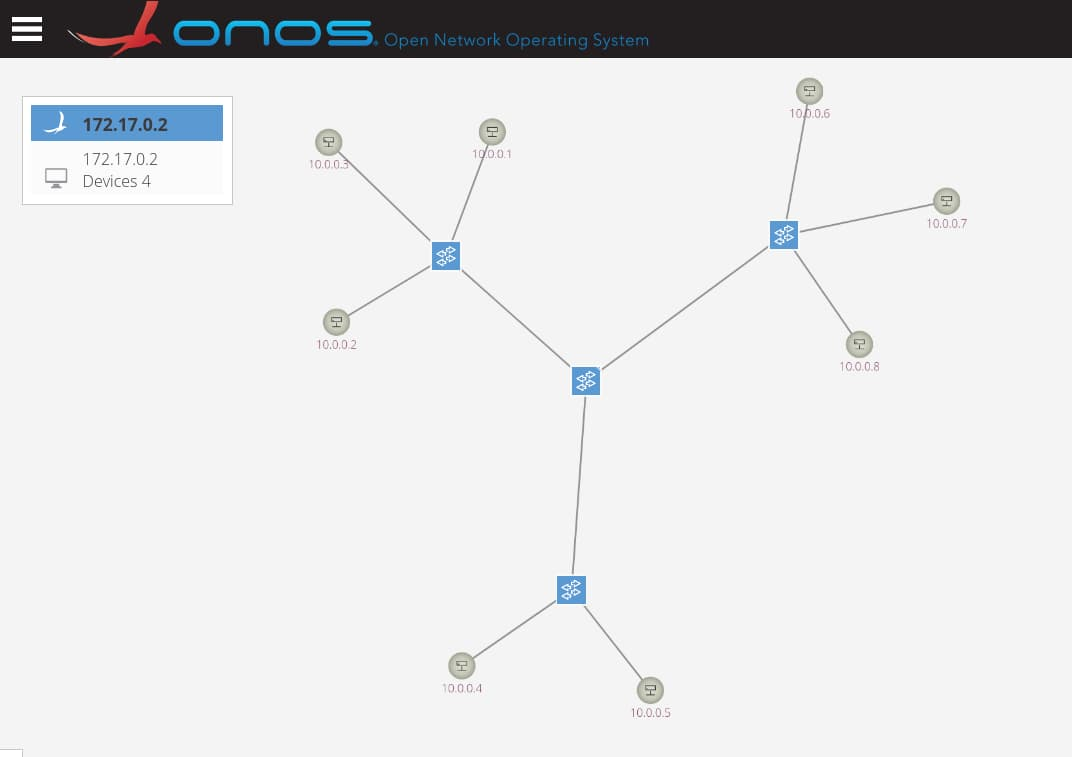
\includegraphics[width=\textwidth]{src/images/chapter4/network-topo.jpg}
    \caption{Mô hình mạng SDN được triển khai tại mỗi zone}
    \label{fig:zone-sdn-topo}
\end{figure}

\subsection{Hệ thống SIEM}

Chúng tôi sử dụng \textit{Wazuh} \footnote{Wazuh: \url{https://wazuh.com}} để tạo nên nền móng cho hệ thống SIEM. Các dữ liệu nguồn gốc trong mạng SDN được thu thập nhờ vào \textit{Wazuh agent}, chúng được cài đặt lên các máy trong mạng, thực hiện giám sát và gửi dữ liệu lên hệ thống SIEM. Bên cạnh đó, \textit{Filebeat} \footnote{Filebeat: \url{https://www.elastic.co/beats/filebeat}} được sử dụng để thu thập và chuẩn hoá dữ liệu flow được gửi từ switch. Các dữ liệu sẽ được lưu trữ và có thể tìm kiếm bởi \textit{Elasticsearch} \footnote{Elasticsearch: \url{https://www.elastic.co/elasticsearch/}}, và cuối cùng sẽ được theo dõi và trực quan hoá nhờ vào \textit{Kibana} \footnote{Kibana: \url{https://www.elastic.co/kibana/}}.
\bigbreak\noindent
Dữ liệu flow được thu thập với định dạng JSON, với mỗi bảng ghi JSON là một flow, bao gồm các thông tin thuộc tính như thông tin của địa chỉ nguồn và đích, kích thước, thời gian, ... Bên cạnh đó dữ liệu nguồn gốc được thu thập bao gồm các sự kiện cũng như các thực thể lưu lại với định dạng JSON, mỗi bản ghi bao gồm các thông tin của mỗi loại thực thể và sự kiện.

\subsection{Hệ thống DPE}

Chúng tôi xây dựng hệ thống này sử dụng công cụ do chúng tôi phát triển nên. Đầu tiên hệ thống sẽ truy vấn lên ElasticSearch để lấy dữ liệu nguồn gốc và các thuộc tính cần thiết của dữ liệu flow cho việc dự đoán được biểu diễn tại bảng~\ref{tab:needed-flow-features} và sẽ được gán bằng 0 nếu các thuộc tính đó không có giá trị xác định khi truy vấn.

\begin{table*}[t]
    \centering
    \caption[Các ràng buộc về thuộc tính cho các quá trình]{Thuộc tính cho dữ liệu flow và ràng buộc của về thuộc tính trong quá trình dự đoán, lưu trữ và truy vấn lên ElasticSearch}
    \label{tab:needed-flow-features}
    \begin{adjustbox}{width=\textwidth}
    \begin{tabular}{|c|c|c|c|c|c|}
    \hline
    \textbf{Thuộc tính} & \textbf{Trường được trích xuất bởi FileBeat} & \textbf{Kích thước} & \textbf{Dự đoán} & \textbf{Lưu trữ} & \textbf{Truy vấn} \\
    \hline
    \texttt{IPV4\_SRC\_ADDR} & \texttt{netflow.source\_ipv4\_address} & 4 bytes  & \texttt{x} & \texttt{x} & \texttt{x} \\
    \hline
    \texttt{IPV4\_DST\_ADDR} & \texttt{netflow.destination\_ipv4\_address} & 4 bytes & \texttt{x} & \texttt{x} & \texttt{x} \\
    \hline
    \texttt{PROTOCOL} & \texttt{netflow.protocol\_identifier} & 1 bytes & \texttt{x} & \texttt{x} & \texttt{x} \\
    \hline
    \texttt{L4\_SRC\_PORT} & \texttt{netflow.source\_transport\_port} & 2 bytes & \texttt{x} & \texttt{x} &  \\
    \hline
    \texttt{L4\_DST\_PORT} & \texttt{netflow.destination\_transport\_port} & 2 bytes & \texttt{x} & \texttt{x} & \\
    \hline
    \texttt{-} & \texttt{netflow.exporter.address} & 4 bytes &  & \texttt{x} &  \\
    \hline
    \texttt{-} & \texttt{netflow.exporter.timestamp} & 4 bytes &  & \texttt{x} &  \\
    \hline
    \texttt{-} & \texttt{netflow.source\_ipv4\_prefix\_length} & 1 bytes & & &  \\
    \hline
    \texttt{-} & \texttt{netflow.destination\_ipv4\_prefix\_length} & 1 bytes & & &  \\
    \hline
    \texttt{IN\_PKTS} & \texttt{netflow.packet\_delta\_count} & 4 bytes & \texttt{x} & & \\
    \hline
    \texttt{OUT\_PKTS} & \texttt{netflow.post\_packet\_delta\_count} & 4 bytes & \texttt{x} & & \\
    \hline
    \texttt{IN\_BYTES} & \texttt{netflow.octet\_delta\_count} & 4 bytes & \texttt{x} & & \\
    \hline
    \texttt{OUT\_BYTES} & \texttt{netflow.post\_octet\_delta\_count} & 4 bytes & \texttt{x} & & \\
    \hline
    \texttt{TCP\_FLAGS} & \texttt{netflow.tcp\_control\_bits} & 1 bytes & \texttt{x} & & \\
    \hline
    \texttt{FLOW\_DURATION\_MILLISECONDS} & \texttt{netflow.flow\_duration\_milliseconds} & 4 bytes & \texttt{x} & & \\
    \hline
    \texttt{L7\_PROTO} & \texttt{netflow.ixia\_l7\_app\_id} & 2 bytes & \texttt{x} & & \\
    \hline
    \end{tabular}
    \end{adjustbox}
\end{table*}

\bigbreak\noindent
Sau khi yêu cầu dự đoán lên hệ thống IDS và nhận lại các dự đoán. Hệ thống DPE sẽ thực hiện ghi các thông tin đó ra một tập tin lưu trữ. Các thông tin được ghi lại gồm một giá trị boolean cho biết là bản ghi flow hoặc các thực thể trong dữ liệu nguồn gốc này có bất thường hay không (chúng tôi chọn giá trị dự đoán lớn hơn $0.5$ sẽ là được cho là bất thường). Với mỗi dự đoán đoán cùng với dữ liệu làm giàu sẽ được lưu lại trong tập tin lưu trữ. Tập tin này sẽ được Wazuh thu thập và phân tích nhằm đưa ra cảnh báo.

\subsection{Hệ thống IDS}

Sau khi được huấn luyện sử dụng học liên kết, các zone sẽ xây dựng một dịch vụ web sử dụng mô hình đã huấn luyện được tạo bởi  Flask\footnote{Flask: \url{https://flask.palletsprojects.com}}, từ đó có thể truy vấn đến và nhận được kết quả dự đoán. Trong quá trình thực nghiệm, hệ thống IDS sẽ nhận dữ liệu flow và đồ thị nguồn gốc đã qua xử lý từ hệ thống tiền xử lý và làm giàu thông tin. Dưới đây là một ví dụ của truy vấn dữ liệu flow lên hệ thống IDS:

\begin{verbatim}
[
    {
        "protocol_identifier": 1,
        "destination_ipv4_address": "10.0.0.4",
        "source_ipv4_address": "10.0.0.1",
        "destination_transport_port": 0,
        "source_transport_port": 0,
        "flow_duration_milliseconds": 10,
        // Các thuộc tính flow khác
    },
    // Các bản ghi flow khác
]
\end{verbatim}

\bigbreak\noindent
Sau đó hệ thống IDS sẽ trả về dự đoán với từng bản ghi đã được gửi lên:

\begin{verbatim}
[
    0.1379,
    // Các dự đoán cho các bản ghi flow khác
]
\end{verbatim}


\section{Đánh giá tính khả thi của mô hình săn tìm APT được hiện thực}

\subsection{Kiểm tra khả năng phát hiện và đưa ra cảnh báo của mô hình thông qua tấn công DoS}

Chúng tôi thực hiện tấn công DoS từ một máy trong mạng SDN có IP là 10.0.0.1 đến máy nạn nhân có IP là 10.0.0.4. Khi cuộc tấn công bắt đầu, các bảng ghi flow trong mạng SDN được thu thập, xử lí, từ đó hệ thống IDS đưa ra dự đoán. Hệ thống IDS phát hiện được rằng có các \textit{flow} bất thường giữa hai IP là 10.0.0.1 và 10.0.0.4 và sau đó đã được ghi \textit{log} lại như \textbf{Hình \ref{fig:evaluation-threat-hunting-ids-detected}}.

\begin{figure}[h]
\centering
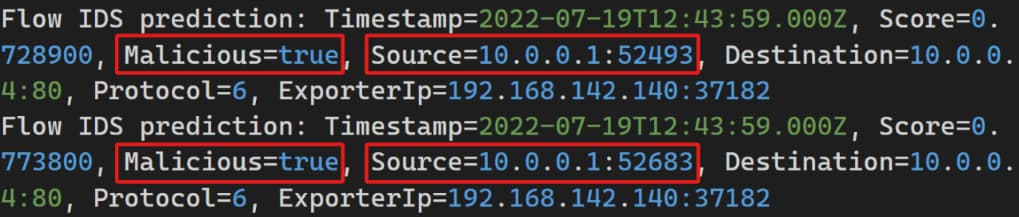
\includegraphics[width=\linewidth]{src/images/chapter4/evaluation-threat-hunting-ids-detected.jpg}
\caption{Dữ liệu từ cuộc tấn công được ghi \textit{log} bởi hệ thống DPE}
\label{fig:evaluation-threat-hunting-ids-detected}
\end{figure}

\bigbreak\noindent
Các dữ liệu này được Wazuh agent thu thập và được lưu trong hệ thống SIEM. Đồng thời hệ thống SIEM cũng đưa ra cảnh báo cho người quản trị như tại \textbf{Hình \ref{fig:evaluation-threat-huntings_wazuh_alert}}, từ đó có thể bắt đầu các cuộc săn tìm lỗ hổng nhằm ngăn chặn cuộc tấn công tiếp diễn.

\begin{figure}[ht]
\centering
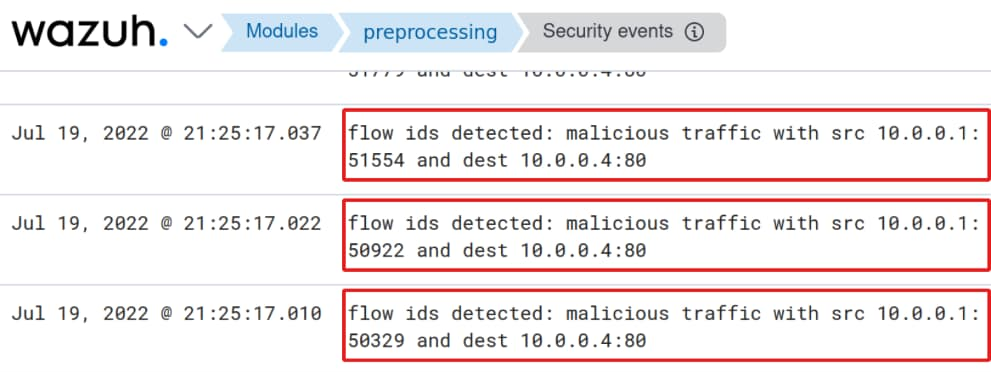
\includegraphics[width=\linewidth]{src/images/chapter4/evaluation-threat-huntings_wazuh_alert.jpg}
\caption{Cảnh báo về cuộc tấn công được hiển thị bởi Wazuh}
\label{fig:evaluation-threat-huntings_wazuh_alert}
\end{figure}

\bigbreak\noindent
Như vậy từ trường hợp này, có thể thấy được hệ thống phát hiện và làm giàu thông tin có khả năng phát hiện và đưa ra cảnh báo với các thông tin hữu ích, phục vụ hiệu quả hơn cho việc thực hiện săn tìm mối đe dọa.

\subsection{Đánh giá hiệu năng của mô hình}
Mô hình được triển khai đã có thể phát hiện được các \textit{flow} bất thường trong mạng SDN, đồng thời, thông tin về được tấn công cũng được tự động làm giàu, ghi \textit{log}, thu thập và trực quan hóa như \textbf{Hình \ref{fig:evaluation-threat-huntings_wazuh_alert}}. Điều này chứng tỏ mô hình có hiệu quả trong triển khai thực tiễn và góp phần giải quyết một phần nào đó vấn đề tự động hóa trong quy trình săn tìm mối đe dọa sự dụng trí tuệ nhân tạo và tăng khả năng diễn giải của các hệ thống IDS sử dụng các mạng nơ-ron phức tạp ở thời điểm hiện tại.

\bigbreak\noindent
Tuy nhiên, Thời gian phản hồi (thời gian Wazuh đưa ra cảnh báo) so với thời gian xuất hiện (thời gian \textit{flow} độc hại xuất hiện trên switch) vẫn còn có sự chênh lệch lớn. Ngoài ra, việc thực hiện tấn công DoS không thể hiện được tính chất của một cuộc tấn công APT nên không thể chứng minh một cách thỏa đáng rằng mô hình triển khai đề xuất có khả năng phát hiện hoặc hỗ trợ phát hiện được các cuộc tấn công APT. Đây là những vấn đề nhóm sẽ cần phải cải tiến và hoàn chỉnh để hoàn thiện mô hình triển khai trong tương lai.

\section{Thảo luận chung}

% trinh bay thao luan chung ve ket qua thuc nghiem thu duoc, neu nhung ket luan tim duoc tu cac so lieu thuc nghiem, phan tich danh gia ve li do dat duoc ket qua

Kết quả thực nghiệm trên hai tập dữ liệu NF-ToN-IoT và DARPA TCE3 đã cho thấy những kết quả đáng kinh ngạc về hiệu suất của mô hình GRU\&CNN và mô hình TGraphSAGE được huấn luyện bằng phương pháp học liên kết FedAvg. Việc sử dụng lớp gộp cực đại toàn cục cho phép mô hình GRU\&CNN vẫn giữ lại được những đặc trưng quan trọng từ các đặc trưng ẩn được trích xuất bởi mô-đun CNN, từ đó loại bỏ bớt tham số cần được huấn luyện nhưng vẫn giữ được độ chính xác của mô hình. Kết quả tương tự xảy ra khi ta thay mô-đun GRU bằng LSTM, tuy nhiên, do LSTM có nhiều tham số hơn GRU nên thời gian cần để huấn luyện biến thể này cũng sẽ tăng lên. Bên cạnh đó, mô hình TGraphSAGE thể hiện hiệu suất ấn tượng nhờ vào sự linh hoạt của mô hình Transformer vượt qua các mô hình được so sánh như doc2vec, word2vec và fasttext trong việc biến đổi đồ thị nguồn gốc với các thuộc tính không cố định về phạm vi giá trị cũng như số lượng thuộc tính thành một đồ thị có thể dễ dàng xử lý bởi mô hình GraphSAGE. Ngoài ra, mô hình Transformer được chúng tôi sử dụng trực tiếp mà không cần phải huấn luyện lại với dữ liệu cục bộ như các mô hình khác nên có thể giảm được nhiều chi phí huấn luyện.
\bigbreak\noindent
Các giải thích được tạo bởi bộ khung SHAP và GNNExplainer cho phép các nhà săn tìm có thể hiểu được dự đoán của các hệ thống IDS thông qua lý giải các nhân tố quan trọng ảnh hưởng đến quyết định của các mạng nơ-ron nhân tạo. Từ các giải thích được trực quan hóa theo nhiều cách (trực quan hóa cho từng giải thích hoặc trực quan hóa cho nhiều giải thích cùng một lúc) của bộ khung SHAP cho các dự đoán của mô hình GRU\&CNN, ta có thể xác định được các thuộc tính ảnh hưởng mạnh đến dự đoán của mô hình GRU\&CNN hoặc xu hướng phân bố độ quan trọng trên các thuộc tính trên một tập các dự đoán. Dựa trên các yếu tố đó, chúng ta có thể đánh giá độ tin cậy của mô hình GRU\&CNN cũng như sử dụng các thông tin trên để phân tích cuộc tấn công đang diễn ra. Bên cạnh đó, giải thích của GNNExplainer cung cấp một đồ thị con tối tiểu gồm các cạnh có độ quan trọng cao đến dự đoán của mô hình GraphSAGE. Với đồ thị con được tạo ra, chúng ta có thể giảm được số nút và cạnh cần phải xác định để đánh giá độ tin cậy của mô hình cũng như quá trình phân tích tấn công. Cuối cùng, phương pháp xác định độ tin cậy của các dự đoán từ các mô hình IDS cung cấp cho chúng ta khả năng đánh giá độ tin cậy của các mô hình một cách tự động thông qua so sánh giá trị đầu ra của lớp áp chót cho dự đoán cần được xem xét với các dự đoán trong lịch sử. Tuy rằng thực nghiệm cho phương pháp được đề xuất đạt kết quả cao, tuy nhiên cần phải được đánh giá thêm bởi sự thiếu hụt trong các mẫu FN và FP. Sự thiếu hụt trên có thể ảnh hưởng rất lớn đến kết quả của phương pháp được đề xuất bởi phương pháp này phụ vào sự gom nhóm của các mẫu và nếu các mẫu quá ít sẽ dẫn đến không đủ thông tin để gom nhóm và không tổng quát hóa được phân bố của các dự đoán. 
\bigbreak\noindent
Cuối cùng, một hệ thống săn tìm tấn công công APT đã được triển khai dựa vào mô hình được đề xuất và chứng minh được khả năng tự động phân tích các hoạt động bất thường và đưa các thông tin về cuộc tấn công đã được làm giàu đến cho các nhà phân tích bảo mật. Tuy nhiên, các thành phần quan trọng khác như: hệ thống CTI, hệ thống diễn giải dự đoán và hệ thống PIDS vẫn chưa được triển khai và đánh giá. Ngoài ra, chúng tôi mô hình chỉ được đánh giá thông qua cuộc tấn công DoS mà không phải một phương pháp đánh giá cụ thể phù hợp để đánh giá tính khả thi và hiệu quả của mô hình trong tấn công APT.
%, cũng như tính khả thi của phương pháp học liên kết FedAvg trong việc đảm bảo hiệu suất huấn luyện các mô hình sử dụng mạng nơ-ron nhân tạo. Từ các giải được tạo bởi bộ khung SHAP và GNNExplainer, hệ thống có thể hỗ trợ cho các nhà săn tìm có thể hiểu được dự đoán của các hệ thống IDS thông qua lý giải các nhân tố quan trọng ảnh hưởng đến quyết định của các mạng nơ-ron nhân tạo. Phương pháp đánh giá độ tin cậy dựa trên đầu ra của lớp áp chót của mạng nơ-ron cũng thể hiện được tiềm năng của mình thông qua kết quả thực hiện. Cuối cùng, chúng tôi triển khai thực tế một hệ thống dựa trên mô hình săn tìm tấn công APT đề xuất và chứng minh khả năng bắt và phân tích một cuộc tấn công thông qua việc thực hiện một cuộc tấn công DoS.
\bigbreak\noindent
Sau toàn bộ quá trình, chúng tôi nhận thấy một số ưu và nhược điểm của mô hình \textbf{XFedHunter} như sau:
\bigbreak\noindent
\textbf{Ưu điểm}
\begin{itemize}
    \item \textit{Giải quyết được bài toán đặt ra:} Đó là hoàn thành mục tiêu đưa AI vào trong các giải pháp săn tìm mối đe dọa thông qua việc xây dựng các hệ thống IDS có hiệu quả cao.

    \item \textit{Giải quyết một số vấn đề khi ứng dụng AI vào săn tìm mối đe dọa:} Như thiếu thông tin từ dự đoán của các mạng nơ-ron nhân tạo, hạn chế trong việc hiểu các quyết định của mạng nơ-ron nhân tạo, không tương thích với các giải pháp bảo mật hiện tại và thiếu sự tự động hóa.

    \item \textit{Mô hình dễ dàng mở rộng}: Sang nhiều tổ chức khác thông qua học liên kết cũng như dễ dàng mở rộng các thành phần trong mô hình săn tìm tấn công APT thông qua việc tách biết các thành phần sử dụng AI và sử dụng cho AI với các giải pháp khác và sự linh động của mạng SDN.
\end{itemize}

\bigbreak\noindent
\textbf{Nhược điểm}
\begin{itemize}

    %\item \textit{Chưa triển khai toàn bộ mô hình săn tìm tấn công APT đề xuất:} Mặc dù chúng tôi đã triển khai được một hệ thống tự động từ lúc thu thập các \textit{flow} trong mạng SDN đến việc đưa ra thông tin làm giàu và dự đoán cho người dùng cuối nhưng hệ thống triển khai vẫn chưa bao gồm các thành phần quan trọng khác như: hệ thống CTI, hệ thống diễn giải dự đoán và hệ thống PIDS.

    \item \textit{Chưa kiểm tra được tính hiệu quả của hệ thống triển khai trong một cuộc tấn công APT thực tế:} Hệ thống triển khai mới được kiểm tra tính khả thi với một cuộc tấn công DoS mà chưa được kiểm tra tính hiệu quả của mô hình bằng một cuộc tấn công APT thực sự.

    \item \textit{Chưa cân nhắc đến trường hợp mất cân bằng dữ liệu khi huấn luyện bằng phương pháp học liên kết:} Chúng tôi phân phối dữ liệu cho các tập huấn luyện cho các máy tham gia liên kết là giống nhau về số lượng mẫu và phân phối giữa tấn công và lành tính. Tuy nhiên, trong thực tế, dữ liệu giữa các bên tham gia sẽ khác nhau về số lượng lẫn phân phối giữa phân phối giữa tấn công và lành tính, các yếu tố này thường có ảnh hưởng không nhỏ đến hiệu suất của mô hình toàn cục nhưng chưa được xem xét trong thực nghiệm của chúng tôi.

    \item \textit{Chưa cân nhắc đến trường hợp tấn công đầu độc khi huấn luyện bằng phương pháp học liên kết:} kiến trúc học liên kết được đề xuất trong \textbf{XFedHunter} có thể bị tấn công đầu độc (poisoning attack) bởi chính các tổ chức tham gia liên kết nếu không có các thao tác xác thực phù hợp trước khi cập nhật mô hình.
\end{itemize}
